%!TEX root =  main.tex
\pagestyle{fancy}
\fancyhf{}
\fancyhead[RE,LO]{\leftmark}
\fancyfoot[CE,CO]{\thepage}
\chapter{Introduction}\label{chapter:Intro}
%
Various software systems have changed the way people communicate, share information, learn, and run businesses. The interconnected computing devices have numerous positive applications in everyday life. In the past decade or so, the volumes of data that is collected, stored, and computed are grown dramatically~\cite{ChiangZ16}. New age applications that might include augmented reality, massive online gaming, face recognition, autonomous drones, and vehicles, or the Internet of Things (IoT) produce enormous amounts of different kinds of data. Such workloads require that latency is below a few tens of milliseconds~\cite{ChiangZ16}, or even less. These requirements fall just right outside of what a standard centralized model like cloud computing (CC), for example, could offer~\cite{ChiangZ16}. Even the smallest problems can contribute to largely unplanned downtime of applications and services people and other services may depend on. A most recent example is yet another outage that was happened to the Amazon Web Services (AWS), and as a result, a large amount of internet becomes unavailable.

This thesis aims to provide formal models based on whom we can model and implement distributed systems (DS) for organizing cloud-like geo-distributed environments for users or CC providers. We can look at the whole system as a micro-cloud or pre-processing layer. The responsibility of such a system is for sending only necessary and data to the cloud. This strategy reduces cost for users and ensuring the availability of CC services. Such a system could lead to lowering the downtime of critical services.

In this section, we are going to give an overview of the topics, that are of significant importance for the rest of the thesis, since it is heavily based on these topics. We start by describing the general problem area that our work addresses in Section~\ref{sec:problem_area}. Sections~\ref{sec:distributed_systems} and \ref{sec:distributed_computing} describe the theoretical background behind the problem, where we examine distributed systems (DS) and distributed computing (DC), focusing on design details, communication patterns, and organizational structure. In Section~\ref{sec:similar_models} we describe similar models that might be a source of confusion, and how they are different than DS or DC, and how some concepts can fit in the bigger picture. Section~\ref{sec:deployment} describe different architecture and application model and how deployment can be done in large DS. In Section~\ref{sec:virtualization_techniques} we describe different virtualization methods that are used in CC for systems and/or applications. In section~\ref{sec:concurency_parallelism} we describe the difference between concurrency and parallelism and introduce an actor system, that will be used later on in the thesis. In Section~\ref{sec:problem_statement}, we specify the exact problem that our work addresses and describe our hypothesis and research goals in Section~\ref{sec:research_hyphotesis_and_golas}. Section~\ref{sec:structure_of_thesis} present the structure of the thesis.
%
%
%
\section{Problem area}\label{sec:problem_area}
%
To lower the administration cost, cloud providers create an effective economy of scale~\cite{BariBEGPRZZ13} by housing data-centers (DCs) with huge capacities. However, such a model does not come with the cost. When such a  system grows to its physical limits, a centralized model brings more harm than good~\cite{GunawiHSLSAE16, LopezMEDHIBFR15}. Despite all the benefits that centralization can provide, it is inevitable for the CC services to suffer from serious problems~\cite{KarimIWGSYO16}. Over time, and due to the high bandwidth and latency, these services face degradation that we cannot overlook. This serious services degradation can have an enormous consequence on the human business and potentially lives as well~\cite{El-SayedSPPGML18}. To avoid large investments~\cite{MonsalveCC18}, like creating and maintaining their own DCs, organizations use cloud services created by others~\cite{Satyanarayanan17}. They consume resources and pay for their usage time. This model is known as -- pay as you go model.

CC requires data transfer to the DCs from data sources. This operation is problematic because it creates a high latency in the system~\cite{HossainRH18}. We can observe few examples like data collection from planes and autonomous cars. Boeing 787s per single flight generates half a terabyte of data, while a self-driving car generates two petabytes of data per single drive. On the other hand, bandwidth is not large enough to support such requirements~\cite{CaoZS18}. Data transfer is not the only problem CC is facing. Some applications require real-time processing for proper decision-making \cite{CaoZS18}. For example, self-driving cars, delivery drones, or power balancing in electric grids. Such applications might face serious issues if a cloud service becomes unavailable due to whatever reson~\cite{GunawiHSLSAE16}.

Over the years, research led to new computing areas and model in which computing and storage utilities are in proximity to data sources~\cite{Satyanarayanan17}. To overcome cloud latency issues centralized CC model is enhanced with some new ideas~\cite{NingLSY20}.
%
%
%
\section{Distributed systems}\label{sec:distributed_systems}
%
There are various definitions of DS, but we can think of DS as a system where multiple entities can communicate to one another in some way, but at the same time, they can perform some operations. In~\cite{SteenT16, 0019513} Tanenbaum et al. give two interesting assumptions about DS:

\begin{enumerate}[start=1,label={(\bfseries \arabic*)}]
	\item  \say{A computing element, which we will generally refer to as a node, can be either a hardware device or a software process}.
	\item \say{A second element is that users (be they people or applications) believe they are dealing with a single system. This means that one way or another the autonomous nodes need to collaborate}.\label{ds:asumption_2}
\end{enumerate}

\noindent
These two assumptions are useful and powerful when talking about DS. As such, in this thesis, we will adopt and use them rigorously.

Three significant characteristics of distributed systems are~\cite{0019513}: 

\begin{enumerate}[start=1,label={(\bfseries \arabic*)}]
	\item \textbf{concurrency of components}, refers to the ability of the DS that multiple activities are executed at the same time. These activities take place on multiple nodes that are part of a DS.
	\item \textbf{independent failure of components}, this property refers to a nasty feature of DS that nodes fail independently. They can fail at the same time as well, but they usually fail independently for numerous reasons.
	\item \textbf{lack of a global clock}, this is a consequence of dealing with independent nodes. Each node has its notion of time, and as such we cannot assume that there is something like a global clock.
\end{enumerate} 

\noindent
In~\cite{SteenT16} authors give formal definition \say{distributed system is a collection of autonomous computing elements that appears to its users as a single coherent system}.

When talking about DS, we usually think about computing systems that are connected via network or over the internet. But DS is not exclusive to the domain of computer science. They existed before computers started to enrich almost every aspect of human life. DS have been used in various different domains such as: \textbf{telecommunication networks}, \textbf{aircraft control systems}, \textbf{industrial control systems} etc. DS are used anywhere where the number of users is growing rapidly so that a single entity cannot respond to the demands in (near) real-time.

Distributed systems (in computer science) are consists of various algorithms, techniques, and trade-offs to create an illusion that a set of nodes act as one. DS algorithms may include: $(1)$ replication, $(2)$ consensus, $(3)$ communication, $(4)$ storage, $(5)$ processing, $(6)$ membership etc.

DS is hard to implement because of its nature. James Gosling and Peter Deutsch both fellows at Sun Microsystems at the time created a list of problems for network applications know as \textit{8 fallacies of Distributed Systems}:\label{enum:fallacies}

\begin{enumerate}[start=1,label={(\bfseries \arabic*)}]\label{ds:8_fallacies}
	\item \textbf{The network is reliable}; there will always be something that goes wrong with the network --- power failure, a cut cable, environmental disasters, etc.
	\item \textbf{Latency is zero}; locally latency is not an issue, but it deteriorates very quickly when you move to the internet and CC scenarios.
	\item \textbf{Bandwidth is infinite}; even though bandwidth is constantly getting better and better, the amount of data we try to push through it rise as well.
	\item \textbf{The network is secure};  Internet attack trends are showing growth, and this becomes a problem even more in public CC.
	\item \textbf{Topology doesn't change}; network topology is usually out of user control, and network topology changes constantly for numerous reasons --- added or removed new devices, servers, breaks, outages, etc.
	\item \textbf{There is one administrator}; nowadays there are numerous administrators for web servers, databases, cache and so one, but also company collaborates with other companies or CC provider.
	\item \textbf{Transport cost is zero}; we have to serialize information and send data over the wire, which takes resources and adds to the total latency. The problem here is not just latency, but that information serialization takes time and resources.
	\item \textbf{The network is homogeneous}; today, a homogeneous network is the exception, rather than a rule. We have different servers, systems, clients that interact. The implication of this is that we have to assume interoperability between these systems sooner or later but we must be aware of it. We might also have some proprietary protocols that might also take time to send on and they may stay without support, so we should avoid them.
\end{enumerate}

\noindent
These fallacies are introduced over a decade ago, and more than four decades since we started building DS, but the characteristics and underlying problems remain pretty the same. It is interesting fact that designers, architects still assume that technology solves everything. This is not the case in DS, and these fallacies should not be forgotten. Because of these problems, DS is hard to implement correctly and they are hard to test and maintain.
%
%
\subsection{Scalability}\label{sec:scalability}
%
Scalability is the property of a system to handle a growing amount of work by adding resources to the system~\cite{Bondi00}. When talking about computer systems scalability can be represented in two flavors:

\begin{itemize}
	\item \textbf{Scaling vertically} means upgrading the hardware that computer systems are running on. Vertical scaling can increase performance to what the latest hardware can offer, and here we are limited by the laws of physics and Moor's law \cite{Gustafson2011}. A typical example that requires this type of scaling is a relation database server. These capabilities are insufficient for moderate to big workloads.
	\item \textbf{Scaling horizontally} means that we scale our system by keep adding more and more computers, rather than upgrading the hardware of a single one. With this approach, we are (almost) limitless on how much we can scale. Whenever performance degrades we can simply add more computers (or nodes). These nodes are not required to be some high-end machines.
\end{itemize}

\noindent
Table~\ref{tab:table1} summarize differences between horizontall and verticall scaling.

\begin{table}[h!]
	\begin{center}
		\begin{tabular}{l|l|l}
			\textbf{Feature} & \textbf{Scaling vertically} & \textbf{Scaling horizontally}\\
			\hline
			\textbf{Scaling} & Limited & Unlimited \\
			\textbf{Managment} & Easy & Comlex\\
			\textbf{Investments} & Expensive & Afordable \\
		\end{tabular}
	\end{center}
	\vspace{-0.5cm}
	\caption{Differences between horizontall and verticall scaling.}
	\label{tab:table1}
\end{table}

\noindent
Scaling horizontally is a preferable way for scaling DS. Not because we can scale easier, or because it is significantly cheaper than vertical scaling (after a certain threshold)~\cite{Bondi00}, but because this approach comes with few more benefits that are especially important when talking about large-scale DS. Adding more nodes gives us two important properties: 

\begin{itemize}
	\item \textbf{Fault tolerance} means that applications running on multiple places at the same time are not bound to the fail of a node, cluster, or even DCs. As long as there is a copy of the application running somewhere, the user will get a response back. As a consequence of running multiple copies of a service and on multiple places, we have that service is more \textbf{avalible}, that running on a single node no matter how high-end that node is. Eventually, all nodes are going to break, and if we have multiple copies of the same service we have a more resilient and more available system to serve user requests.
	\item \textbf{Low latency} refers to the idea that the world is limited by the speed of light. If a node running application is too far away, the user will wait too long for the response to get back. If the same application is running in multiple places, the user request will hit the node that is closest to the user.
\end{itemize}

\noindent
But despite all the obvious benefits, for a DS to work properly, we need the writing software in such a way that is able to run on multiple nodes, as well as that accept \textbf{failure} and deal with it. This turns out to be not an easy task.

For example, users need to be aware when using DS, which is related to distributed data storage systems. Storage implementations that rely on vertical scaling to ensure scalability and fault tolerance, have one nasty feature. 

This nasty feature is represented in theorem called \textbf{CAP theorem} presented by Eric Brewer~\cite{Brewer2000}, and proven after inspection by Gilbert et a.~\cite{GilbertL02}. The CAP theorem states that it is impossible for a distributed data store to simultaneously provide more than two out of three guarantees shown in Figure~\ref{fig:fig17}.

\begin{figure}[H]
	\begin{center}
		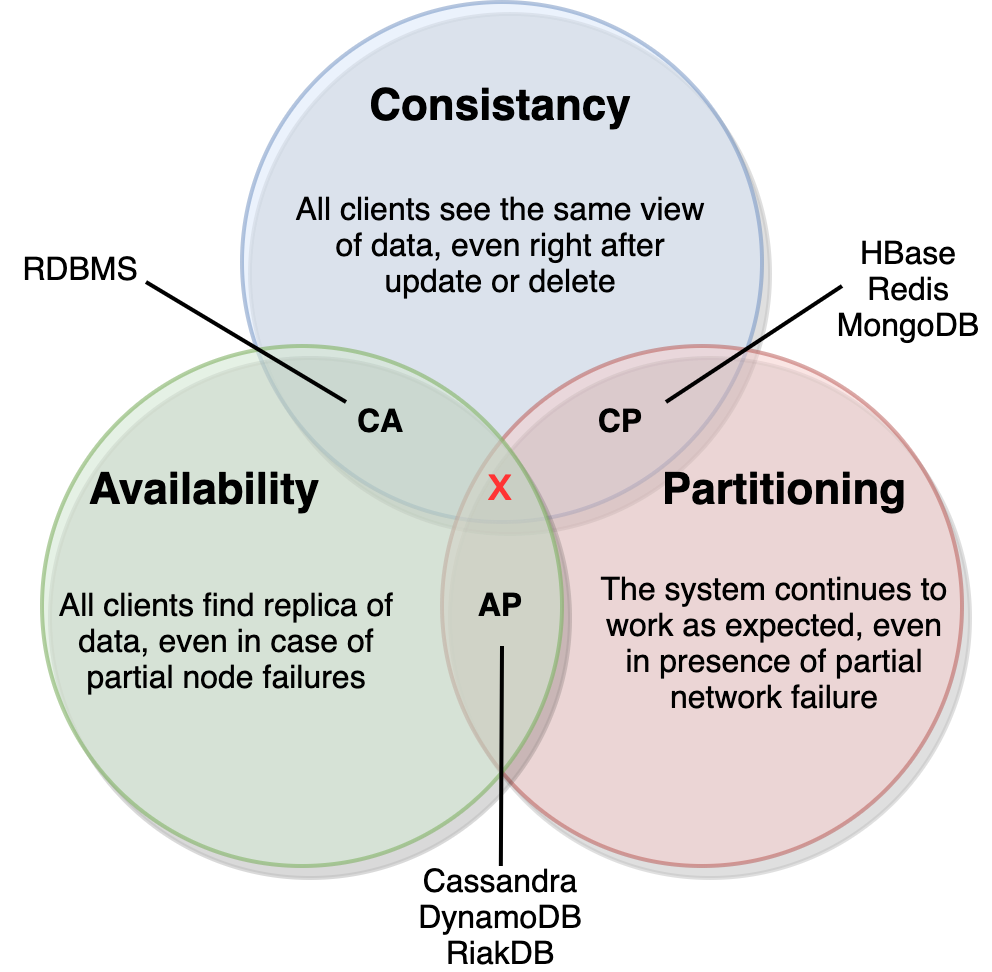
\includegraphics[scale=0.9]{images/Figure17.png}
	\end{center}
	\vspace{-0.6cm}
	\caption{Difference between cloud options and on-premises solution.}
	\label{fig:fig17}
\end{figure}

\begin{enumerate} [start=1,label={(\bfseries \arabic*)}]
	\item \textbf{C}onsistency, which means that all clients will see the same data at the same time, no matter which node they are connected to. Clients may not be connected to the same node since data could be replicated on many nodes in different locations.
	\item \textbf{A}vailability, which means that any client issued a request will get a response back, even if one or nodes are down. DS will not interpret this situation as an exception or error. Availability is represented in percentage, and it describes how much downtime is allowed per year, This can be calculated using formula:\\ 
	
	\begin{equation}\label{eq:Availability}
		Availability = \frac{uptime}{ (uptime + downtime)}
	\end{equation}
	\myequations{Availability percentage formula}
	The industry is using measuring availability in \say{class of nines}. Availability class is the number of leading nines in the availability figure for a system or module~\cite{GrayS91}. This metric relates to the amount of time (per year) that service is up and running. Table~\ref{tab:table7} show different classes of nine and their availability and unavailability in minutes per year (\textbf{min/year}) for some examples~\cite{GrayS91}.
	
	\begin{table}[h!]
		\begin{center}
			\begin{tabular}{l|l|l}
				\textbf{Type} & \textbf{Availability} & \textbf{Unavailability} \\
				\hline
				\textbf{Unmanaged} & 90\% & 50,000 \\
				\textbf{Managed} & 99\% & 5,000 \\
				\textbf{Well-managed} & 99.9\% & 500 \\
				\textbf{Well-managed} & 99.9\% & 500 \\
				\textbf{Fault-tolerant} & 99.99\% & 50 \\
				\textbf{High-availability} & 99.999\% & 5 \\
				\textbf{Very-high-availability} & 99.9999\% & 0.5 \\
			\end{tabular}
		\end{center}
		\vspace{-0.5cm}
		\caption{Downtime for different classes of nines.}
		\label{tab:table7}
	\end{table}
	
	\noindent
	We can calculate availability class if we have system availability $A$, the system's availability class is defined as~\cite{GrayS91}: 
	
	\begin{equation} 
		e^{\log_{10} \frac{1}{ (1 - A)}} 
	\end{equation}
	\myequations{Availability class formula.}
	It is important to notice that even a 99\% available system gives almost four days of downtime in a year, which is unacceptable for services like Facebook, Google, AWS, etc. And when service is down, companies are losing customers.
	\item \textbf{P}artition tolerance, which means that the cluster must continue to work despite any number of communication breakdowns between nodes in the system. It is important to state that in a distributed system, partitions cannot be avoided.
\end{enumerate}

\noindent
Years after CAP theorem inception, Shapiro et al. prove that we can alleviate CAP theorem problems, but only in some cases, and offers \textbf{Strong Eventual Consistency (SEC) model}~\cite{ShapiroPBZ11}. They prove that if we can represent our data structure to be: \label{crdts}

\begin{itemize}
	\item \textbf{Commutative} $a*b = b*a$ \myequations{Commutative formula.}
	\item \textbf{Associative} $(a*b)*c = a*(b*c)$ \myequations{Associative formula.}
	\item \textbf{Idempotent} $(a * a) = a$ \myequations{Idempotent formula.}
\end{itemize}

\noindent
where $*$ is a binary operation, for example: $max$, $union$, $or$ we can rely on SEC properties,
%
%
\subsection{Cloud computing}\label{sec:cloud_computing}
%
Vogels et al. describe CC as an \say{aggregation of computing resources as a utility, and software as a service}~\cite{Vogels}.  Big DCs provide hardware and software services for their users over the internet~\cite{AboveTheCloud}. Cloud providers offer various resources like CPU, GPU, storage, and network as utilities that can be used and released on-demand~\cite{ZhangCB10}. The key strength of the CC is reflected in the offered services~\cite{Vogels}. To support the various application needs, the traditional CC model provides enormous computing and storage resources elastically. This property refers to the cloud ability to allow services to allocate additional resources or release unused ones to match the application workloads on-demand~\cite{AssuncaoVB18}. Services usually fall in one of three main categories: 

\begin{itemize}
	\item \textbf{Infrastructure as a service (IaaS)} allows businesses to purchase resources on-demand and as-needed instead of buying and managing hardware themself;
	\item \textbf{Platform as a service (PaaS)} delivers a framework for developers to create, maintain and manage their applications. All resources are managed by the enterprise or a third-party vendor;
	\item \textbf{Software as a service (SaaS)} deliver applications over the internet to its users. These applications are managed by a third-party vendor;
\end{itemize}

\noindent
Figure~\ref{fig:fig1} show the difference in control and management of resources between different cloud options and on-premises solutions.

\begin{figure}[H]
	\begin{center}
		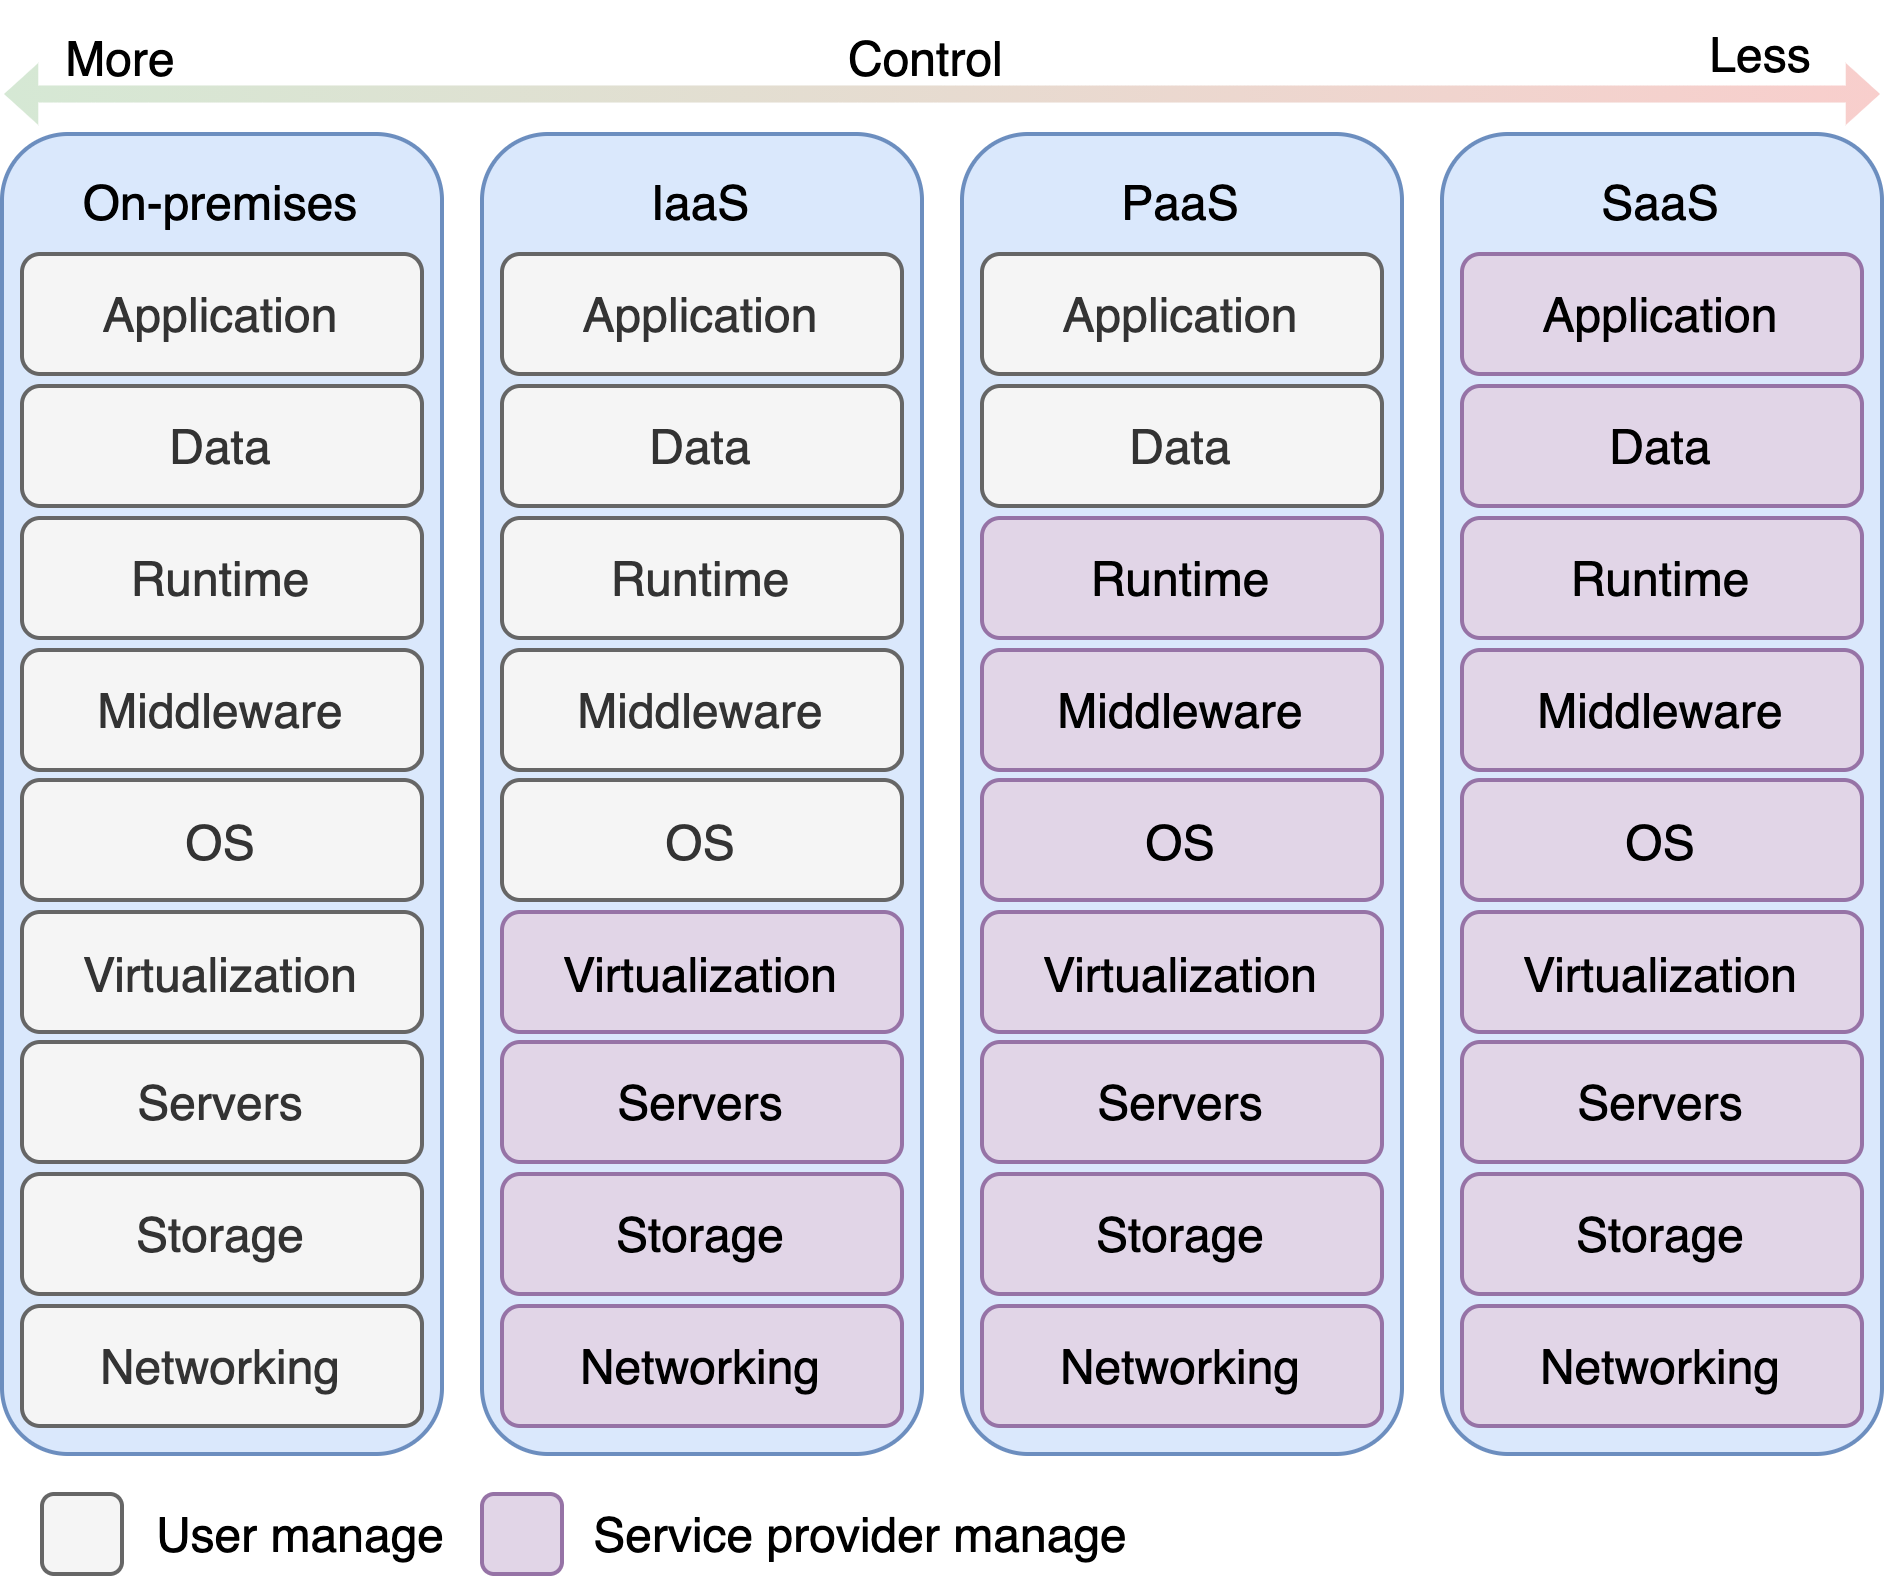
\includegraphics[scale=0.9]{images/Figure1.png}
	\end{center}
	\vspace{-0.6cm}
	\caption{Difference between cloud options and on-premises solution.}
	\label{fig:fig1}
\end{figure}

\noindent
The user can choose a single solution, or combine more of them if such a thing is required depending on preferences and needs.

By the ownership, CC can be categorized into three categories:

\begin{itemize}
	\item \textbf{Public cloud} is a type where CC is delivered over the internet and shared across many many organizations and users. In this type of CC, architecture is built and maintained by others. Users and organizations pay for what they use. Examples include AWS EC2, Google App Engine, Microsoft Azure, etc.
	\item \textbf{Private cloud} is a type where CC is dedicated only to a single organization. In this type of CC, architecture is built by an organization that may offer their solution or services to the users or other organizations. These services are in the domain of what the organization does, and that organization is in charge of maintenance. Examples include VMWare, XEN, KVM, etc.
	\item \textbf{Hybrid cloud} in such an environment that uses both public and private clouds. Examples include IBM, HP, VMWare vCloud, etc.
\end{itemize}

\noindent
Table~\ref{tab:table4} show comparison of public, private and hybrid cloud capabilities.\label{sec_types}

\begin{table}[h!]
	\begin{center}
		\begin{tabular}{l|l|l|l}
			\textbf{Capabilities} & \textbf{Public cloud} & \textbf{Private cloud} & \textbf{Hybrid cloud}\\
			\hline
			\textbf{Data control} & IT enterprise & Service Provider & Both \\
			\textbf{Cost} & Low & High & Moderate \\
			\textbf{Data security} & Low & High & Moderate \\
			\textbf{Service levels} & IT specific & Provider specific & Aggregate \\
			\textbf{Scalability} & Very high & Limited & Very high \\	
			\textbf{Reliability} & Moderate & Very high & Medium/High\\	
			\textbf{Performance} & Low/Medium & Good & Good \\
\end{tabular}
	\end{center}
	\vspace{-0.5cm}
	\caption{Comparison of public, private and hybrid cloud capabilities.}
	\label{tab:table4}
\end{table}

\noindent
In the rest of the thesis, if not stated differently when CC term is used it denotes public cloud.

CC has been the dominating tool in the past decade in various applications~\cite{Satyanarayanan17}. It is changing, evolving, and offering new types of services. Resources such as container as a service (CaaS), database as a service (DBaaS)~\cite{Peter} are newly introduced. The CC model gives us a few benefits. Centralization relies on the economy of scale to lower the cost of administration of big DCs. Organizations using cloud services avoid huge investments. Like creating and maintaining their own DCs. They consume resources usually created by others~\cite{Satyanarayanan17} and pay for usage time -- pay as you go model. 

But centralization gives us few really hard problems to solve. As already stated in section~\ref{sec:problem_area} data is required to be moved to the cloud from data sources, which introduces a high latency in the system~\cite{HossainRH18}. 

There are few notable attempts to help data ingestion into the cloud. Remote Direct Memory Access (RDMA) protocol makes it possible to read data directly from the memory of one computer and write that data directly to the memory of another. This is done by using \textit{specialized hardware} interface cards and switches and software as well, and operations like reading, write, send, receive, etc. do not go through the CPU. With these characteristics, RDMA has low latencies and overhead, and as such reaches better throughputs~\cite{CohenTKCKRCDG09}. This new hardware may not be cheap, and not every CC provider uses them for every use-case. And this may not be enough, especially with the ever-growing amount of IoT devices and services.

Over the years there are more service options available, forming \textbf{everything as a service (XaaS)} model~\cite{DuanFZSNH15}. This model proposes that any hardware or software resource can be offered as a service to the users over the internet.

Table~\ref{tab:table2} shows common examples of SaaS, PaaS, and IaaS applications.

\begin{table}[h!]
	\begin{center}
		\begin{tabular}{l|l}
			\textbf{Platform} & \textbf{Common Examples}\\
			\hline
			\textbf{IaaS} & AWS, Microsoft Azure, Google Compute Engine \\
			\textbf{PaaS} & AWS Elastic Beanstalk, Azure, App Engine \\
			\textbf{SaaS} & Gmail, Dropbox, Salesforce, GoToMeeting \\
		\end{tabular}
	\end{center}
	\vspace{-0.5cm}
	\caption{Common examples of SaaS, PaaS, and IaaS.}
	\label{tab:table2}
\end{table}

\noindent
In recent years there is one extension of CC from a series standpoint called \textbf{multi-cloud}~\cite{HongDSH19, Ardagna15}. 

A multi-cloud environment is a such environment where an enterprise uses more than one cloud platform, with at least two or more public cloud providers, that each delivers a specific application or service. A multi-cloud can be comprised of any model presented on page~\pageref{sec_types}. This model relies on the possibility that if one cloud provider fails for whatever reason, the next one will be able to serve user requests.

CC is giving a user an illusion that he is using a single machine, while the background implementation is fairly complicated and consists of various elements that are composed of countless machines. CC is a typical example of a horizontally scalable system presented in~\ref{sec:scalability}.
%
%
\subsection{Membership protocol}\label{sec:memership_protocol}
%
A the start of this section we introduced DS, and we present two interesting assumptions by Tanenbaum et al.~\cite{SteenT16, 0019513}. If we take one more look at the~\ref{ds:asumption_2} assumption, we will see that users of the DS whether they are users or applications perceive DS as a single unit. Inside this single unit, nodes need to collaborate, so that they are able to do various kinds of tasks.

The most basic of all these tasks is that nodes need to know which group they belong to, and who are their peers in the group they will collaborate with. This might sound like a trivial idea, but when we include 8 fallacies of the DS~\ref{ds:8_fallacies} into the equation, things start to be not so trivial, after all. In the setup where nodes are connected over the local network or internet, and they need to communicate things will go wrong for various reasons.

To resolve the problem that nodes need to know who are their group peers, a membership protocol comes to help. These protocols need to ensures that each process of one group updates its local list of \textbf{non-faulty} members of the group, and when a new process joins or leaves the group, the local list for every process needs to be updated. This is the most basic idea behind membership protocols.

Processes in the group of nodes in a group will ping each other in different ways, and using different strategies to figure out which nodes are dead and which are alive. There are few existing algorithms that do this job, and they are (usually) based on the way epidemics spread or how gossip is spread in a human population. Because of this feature, these algorithms are usually called \textit{Gossip} style protocols.

Every membership protocol has some properties that will ensure efficiency and scalability:

\begin{enumerate}[start=1,label={(\bfseries \arabic*)}] \label{ds:features}
	\item \textbf{Completeness}, this property must ensure that every failure in the system is detected.
	\item \textbf{Accuracy}, in an ideal world, there should be no mistakes when detecting failures. But In a real-life scenario, we need to reduce false positives as much as we can.
	\item \textbf{Failure detection speed}, all failures needs to be treated as fast as possible, in order to remove the node from the group and reschedule the tasks from dead node to alive ones.
	\item \textbf{Scale}, with this property we must ensure that the network load that is generated should be distributed equally between all processes in the group.
\end{enumerate}

\noindent
The easiest idea to implement this protocol would be \textbf{heartbeating} technique where process $P_i$ will send a heartbeat message to all his peers in the group or \textbf{multicast}. After some time if process $P_j$ did not receive a heartbeat message from $P_i$, it will mark him as failed. This idea is easy to understand, and implement but the downsides are that his process is not that \textbf{scalable}, especially for large groups, and this will introduce huge network traffic.

To resolve this problem, Das et al.~\cite{DasGM02} introduced \textbf{S}calable \textbf{W}eakly-consistent \textbf{I}nfection-style Process Group \textbf{M}embership protocol, or \textbf{SWIM} for short\label{swim}. This protocol divides the membership problem into two parts:

\begin{enumerate}[start=1,label={(\bfseries \arabic*)}]
	\item \textbf{Failure detection}, this component works so that one node will select a random node in the group, and it will send him $ping$ message, expecting $ack$ message in return --- \textbf{direct ping}. If such message is not received, he will pick $n$ nodes to probe through a $ping-req$ message --- \textbf{indirect ping}. If this fails, the node will be marked as $suspected$, and it will be marked as $dead$ after some timeout. If the node gets alive, he will ping some other node and he will get back into the group. Figure~\ref{fig:fig15} show message passing in \textbf{direct} $(left)$, and \textbf{indirect} $(right)$ ping in SWIM protocol.
	\item \textbf{Information dissemination}, with previous strategy, we can disseminate information by \textbf{piggybacking} the data on multiple messages ($ping$, $ping-req$ and $ack$), and avoid using the multicast solution.
\end{enumerate}

\begin{figure}[H]
	\begin{center}
		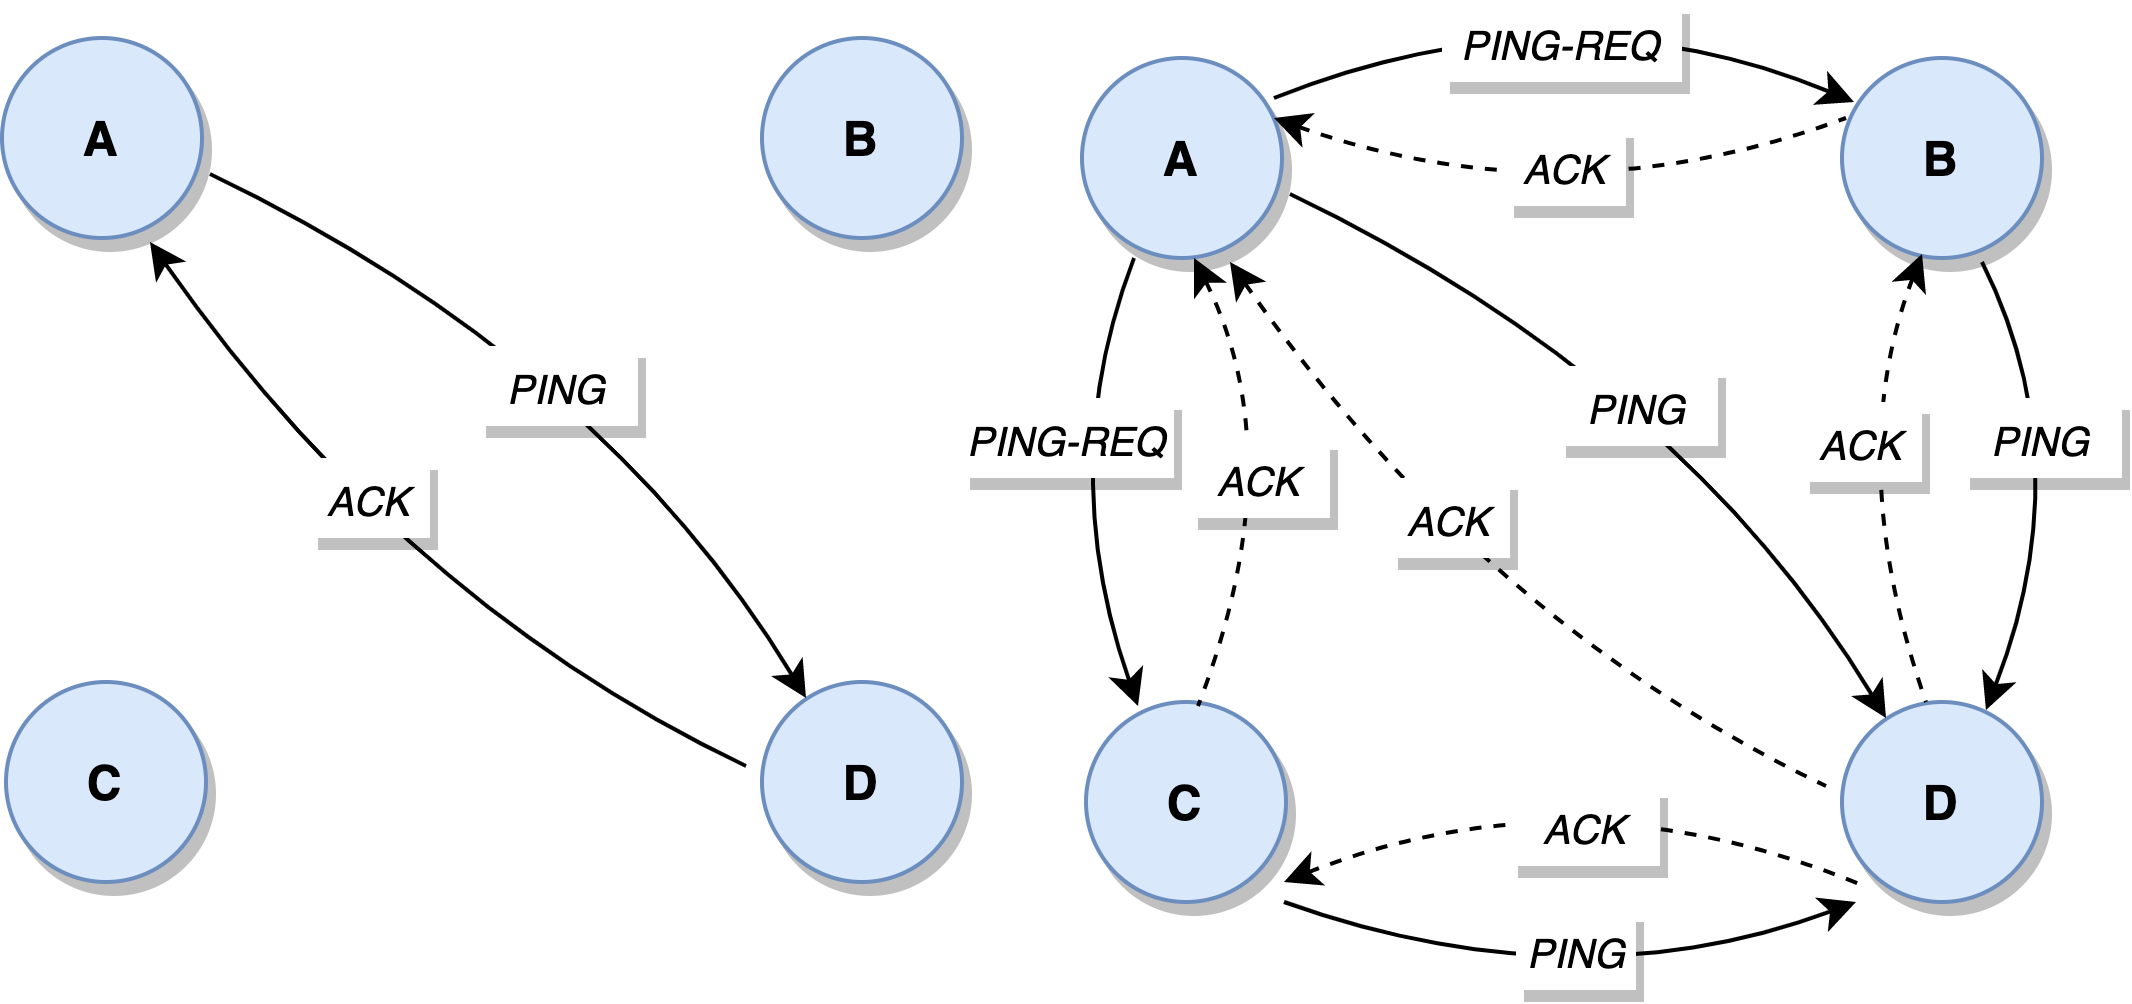
\includegraphics[scale=0.7]{images/Figure15.png}
	\end{center}
	\vspace{-0.6cm}
	\caption{Direct and indirect ping in SWIM protocol.}
	\label{fig:fig15}
\end{figure}

\noindent
Over the years, researchers found ways to improve the protocol for example Dadgar et al. present Lifeguard protocol~\cite{DadgarPC18} for more accurate failure detection, and there are other implementations to fine-tune the SWIM, but the base idea is still there. Today SWIM or SWIM-like protocols are standard membership protocols whenever we are doing some node clustering.
%
%
\subsection{Mobile computing}\label{sec:mobile_computing}
%
The first idea that introduced task offloading from the cloud~\cite{FernandoLR13, LinLJL19} was Mobile cloud computing (MCC). The mobile devices run small client software and interact with the cloud over the internet, while heavy computation remains in the cloud. 

The cloud is usually far away from end devices because DCs are built on specific locations in the world to target as many users nearby as possible. This sparse deployment will most likely lead to high latency, and bad quality of experience (QoE)~\cite{LinLJL19} for most users. Latency-sensitive applications especially will have a hard time. As a model, MCC is not much different from the standard CC model. The good thing is that we relaxed the cloud a little bit, and We had moved a small number of tasks from the cloud. But this model opens the door for the next-generation models.

The development led to new computing areas like edge computing (EC). EC is a next-generation model where computing and storage resources are in proximity to data sources~\cite{Satyanarayanan17}. This idea might overcome cloud latency issues and known MCC problems. The main strength of the EC lays in the CC enhancements with new processing ideas, for the next-generation use-cases~\cite{NingLSY20}. 

EC brought few different models over the years. Models like fog~\cite{BonomiMNZ14}, cloudlets~\cite{MonsalveCC18}, and mobile edge computing (MEC)~\cite{WangZZWYW17} emerged. This thesis will refer to all these models as edge nodes. Different EC models rely on the concept of data and computation offloading from the cloud closer to the ground~\cite{KhuneP19}. Only heavy computation remains in the cloud because of more available resources~\cite{NingLSY20}, compared to edge nodes. 

EC models introduced small-scale servers that operate between data sources and the cloud. These small-scale servers have much fewer capabilities compared to the cloud servers~\cite{ChenHLLW15}. To avoid latency and huge bandwidth~\cite{MonsalveCC18}, EC nodes can be dispersed in various locations, for example, base stations~\cite{WangZZWYW17}, coffee shops, or over arbitrary geographic regions.
%
%
\section{Distributed computing}\label{sec:distributed_computing}
%
Distributed computing (DC) can be defined as the use of a DS to solve one large problem by breaking it down into several smaller parts, where each part is computed in the individual node of the DS and coordination is done by passing messages to one another~\cite{0019513}. Computer programs that use this strategy and runs on DS are called \textbf{distributed programs} \cite{Vera16, andrews2000foundations}. 

Similar to CC in Section~\ref{sec:cloud_computing}, to a normal user, DC systems appear as a single system similar to one he uses every day on his personal computer. DC shares the same fallacies to DS presented in~\ref{sec:distributed_systems}.
%
%
\subsection{Big Data}\label{sec:big_data}
%
Term big data means that the data is unable to be handled, processed, or loaded into a single machine~\cite{FisherDCD12}. That means that traditional data mining methods or data analytics tools developed for centralized processing may not be able to be applied directly to big data~\cite{Tsai2015}. 

New tools and methods that are developed are relying on DS and one specific feature \textbf{data locality}~\label{ds:data_locality}. Data locality can be described as a process of moving the computation closer to the data, instead of moving large data to computation~\cite{GuoFZ12}. This simple idea minimizes network congestion and increases the overall throughput of the system.

In~\ref{sec:problem_area} we already give two examples of how huge generated data could be, and when we include other IoT sensors and devices these numbers will just keep getting bigger~\cite{SarigiannidisLR20}.

On contrary to relational databases that mostly deal with structured data, big data is dealing with various kinds of data~\cite{FisherDCD12, Tsai2015, GuoFZ12}:

\begin{itemize}
	\item \textbf{Structured} data is a kind of data that have some fixed structure and format. A typical example of this is data stored inside a table of some database. organizations usually have no huge problem extracting some kind of value out of the data.
	\item \textbf{Unstructured} data is a kind of data where we do not have any kind of structure at all. These data sources are heterogeneous and may contain a combination of simple text files, images, videos, etc. This type of data is usually in raw format, and organizations have a hard time deriving value out.
	\item \textbf{Semi-structured} data is the kind of data that can contain both previously mentioned types of data. An example of this type of data is XML files.
\end{itemize}

\noindent
Along with the share size, big data have other instantly recognizable features called \textbf{V's} of big data~\cite{PatgiriA16}. Name is derived from starting letters from the other features that are describing big data. Image~\ref{fig:fig3} show 6 V's commonly used to represent the big data.

\begin{figure}[H]
	\begin{center}
		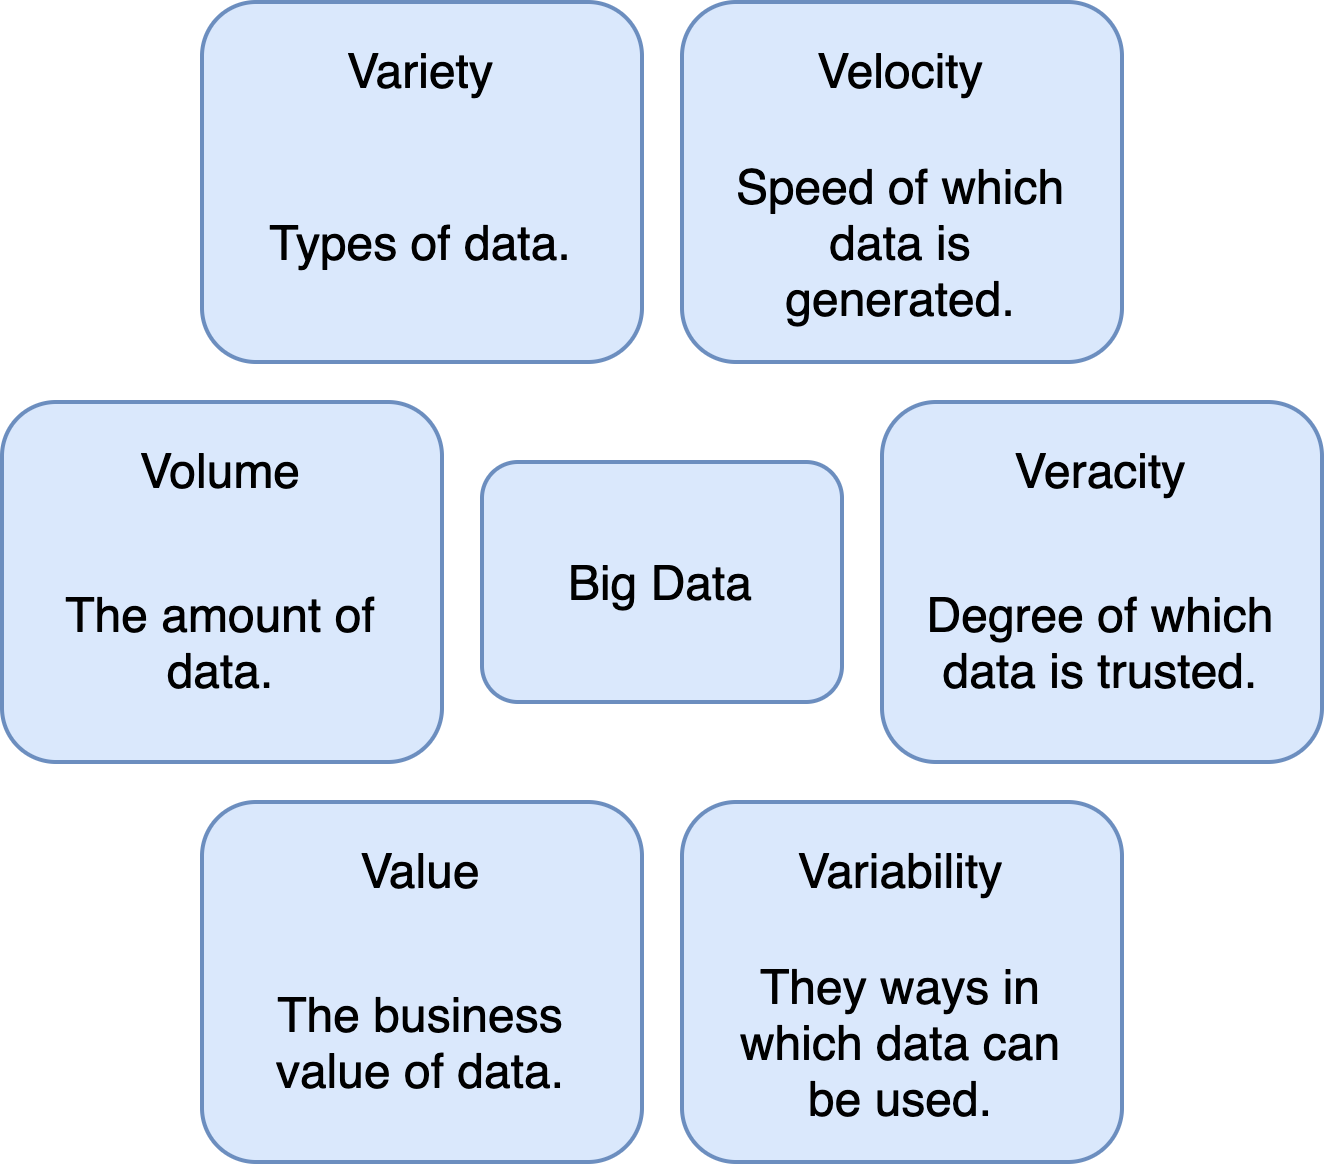
\includegraphics[scale=0.7]{images/Figure3.png}
	\end{center}
	\vspace{-0.6cm}
	\caption{V's of Big Data.}
	\label{fig:fig3}
\end{figure}

\noindent
Processing in big data systems can be represented as~\cite{phdthesis, KiranMMDB15}:

\begin{itemize}
	\item \textbf{Batch processing} represents a data processing technique that is done on a huge quantity of the stored data. This type of processing is usually slow and requires time.
	\item \textbf{Stream processing} represents a data processing technique that is done as data get into the system. This type of processing is usually done on a smaller quantity of the data \textbf{at the time}, and it is faster.
	\item \textbf{Lambda architectures} represents a processing technique where stream processing and handling of massive data volumes in a batch are combined in a uniform manner, reducing costs in the process~\cite{KiranMMDB15}.
\end{itemize}

\noindent
Big data systems, are not processing and value extracting systems. Big data systems can be separated into few categories: $(1)$ data storage, $(2)$, data ingestion $(3)$, data processing, and analytics. All these systems aids to properly analyze ever-growing requirements~\cite{RaoMBG19},

Despite a promise that big data offers to derive value out of the collected data, this task is not easy to do and requires properly set up system filtering and removing data that contains no value. To aid this idea, data could be filtered and a little bit preprocessed on close to the source~\cite{inproceedingsSimic1}, and as such sent to data lakses~\cite{MarynowskiSP15}.
%
%
\subsection{Microservices}\label{sec:microservices}
%
There is no single comprehensive definition of what a microservice is. Different people and organizations use different definitions to describe them. A working definition is offered in~\cite{DragoniGLMMMS16} as~\say{s microservice is a cohesive, independent process interacting via messages}. Despite the lack of a comprehensive definition, all agree on few features that come with microservices:

\begin{enumerate}[start=1,label={(\bfseries \arabic*)}]
	\item they are small computer programs that are independently deployable and developed.
	\item they could be developed using different languages, principles, and using different databases.
	\item they communicate over the network to achieve some goal.
	\item they are organized around business capabilities~\cite{PautassoZALJ17}.
	\item they are implemented and maintained by a small team.
\end{enumerate}

'\noindent
The industry is migrating much of their applications to the cloud because CC offers to scale their computing resources as per their usage~\cite{LiZJLZLGGS19}. Microservices are small loosely coupled services that follow UNIX philosophy~\say{do one thing and do it well}~\cite{krause2015microservices}, and they communicate over well defined API~\cite{DragoniGLMMMS16}.

This architecture pattern is well aligned to the CC paradigm~\cite{LiZJLZLGGS19}, contrary to previous models like monolith whose modules cannot be executed independently~\cite{DragoniGLMMMS16, abs-1905-07997}, and are not well aligned with the CC paradigm~\cite{abs-1905-07997}. Table~\ref{tab:table3} summarize differences between the monolith and microservices architecture.

\begin{table}[h!]
	\begin{center}
		\begin{tabular}{l|l|l}
			\textbf{Feature} & \textbf{Monolith} & \textbf{Microservices}\\
			\hline
			\textbf{Structure} & Single unit & Independent services \\
			\textbf{Management} & Usually easier & Add DS complexity\\
			\textbf{Scale/Update} & Entire app & Per service \\
			\textbf{Error} & Usually crush entire app & App continue to work \\
		\end{tabular}
	\end{center}
	\vspace{-0.5cm}
	\caption{Differences between horizontall and verticall scaling.}
	\label{tab:table3}
\end{table}

\noindent
Since its inception, microservices architecture is gone through some adaptations. And modern-day microservices are extended with two new models each with its unique abilities and problems:

\begin{itemize}
	\item \textbf{Cloud-native applications} are specially designed applications for CC. They are distributed, elastic, and horizontally scalable systems by their nature, and composed of (micro)services that isolate state in a minimum of stateful components~\cite{KratzkeQ17}. These type of applications are self-contained, could be deployed independently, and they are composed of loosely coupled microservices that are packaged in lightweight containers. They have Improved resource utilization, and they are centered around APIs.
	\item \textbf{Serversles applications} is a computing model, where the developers need to worry only about the logic for processing client requests~\cite{AdzicC17}. Logic is represented as an event handler that only runs when a client request is received, and billing is done only when these functions are executing~\cite{AdzicC17}. \textbf{Cold start} is one of the features of serverless computing, and we can define it as user requests need to wait until a new container instance is up and running before can do any processing at all. Most providers have 1–3 second cold starts, and this is important for certain types of applications where latency is a concern. Cold start is only happening when there are no \textit{warm} containers available for the request, meaning there is no single instance to server request. Other features include: $(1)$ simplified services development, $(2)$ faster time to market, $(3)$ and lower costs.
	\item \textbf{Service Mesh} is designed to standardize the runtime operations of applications~\cite{LiLGZH19}. As part of the microservices ecosystem, this dedicated communication layer can provide several benefits, such as: $(1)$ observability, $(2)$ providing secure connections, or $(3)$ automating retries and backoff for failed requests. With these features, developers only focus on the implementation of business logic, while operators gain out-of-the-box traffic policies, observability, and insights from the services. Advocates of the microservice movement, nowadays recommend using service mesh architecture when running microservices in production environments.
\end{itemize}

\noindent
Previous models are not explicitly different, they all can be viewed as cloud-native applications. The enumeration is given for the sake of pointing out their different models and aspects of working.

Microservices communicate over a network to fulfill some goal using message passing techniques and technology-agnostic protocols such as HTTP. They can be implemented as:

\begin{itemize}
	\item Representational state transfer (REST) services~\cite{AdamczykSJH11}, is an architectural style with a set of constraints that users can create web services and interoperability between computer systems on the internet. It is based on HTTP routs to define resources and used HTTP verbs to represent operations over these resources. It relies on textual based communications, and payload could be represented using $JSON$, $XML$, $HTML$ etc.
	\item Remote procedure calls (RPC) represent an architectural way to design services that can call subroutines that are located in different places, usually on another machine. The client is calling these operations like they are located locally in his address space.
	\item Event-driven services are services where communication between services is done using events. Events are sent on some channel and other read messages that are received on another channel. These channels could be implemented either like message queues or message topics. Services connect to message queue or subscribe to the specific topic, and when messages arrive, they can act according to the message type.
\end{itemize}
 
\noindent
They are well aligned with text-based protocols like HTTP/1 using $JSON$ for example, or binary protocols such as HTTP/2 using $protobuf$ and $gRPC$ for example, and even new faster version like HTTP/3 over new $QUIC$ protocol, designed by Google. HTTP 3 is the latest version of the conventional and trusted HTTP protocol. It is very similar to HTTP 2, but it also offers a few important new features. Table~\ref{tab:table9} show important difference between versions of HTTP protocol.
 
 \begin{table}[h!]
 	\begin{center}
 		\begin{tabular}{l|l|l|l}
 			\textbf{Feature} & \textbf{HTTP1} & \textbf{HTTP2} & \textbf{HTTP3}\\
 			\hline
 			\textbf{Transport} & text & binary & binary\\
 			\textbf{Parallelism} & No & Yes & Yes\\
 			\textbf{Protocol} & TCP & TCP & QUIC \\
 			\textbf{Space} & OS level & OS level & User level\\
 			\textbf{Server push} & No & Yes & Yes\\
 			\textbf{Compression} & Data & Data/Headers & Data/Headers\\
 		\end{tabular}
 	\end{center}
 	\vspace{-0.5cm}
 	\caption{Idempotent and non-idempotent operations.}
 	\label{tab:table9}
 \end{table}
 
\noindent
To ensure a wider range of devices that can communicate with the rest of the systems, developers usually have a gateway into the system that is REST service, and other services could be implemented differently.

It is important to point out, that all flavors of microservices applications rely on continuous delivery and deployment~\cite{7436659}. This is enabled by lightweight containers, instead of virtual machines~\cite{FelterFRR15}, and orchestration tools such Kubernetes~\cite{BurnsGOBW16}. These concepts will be described in more detail in Section~\ref{sec:virtualization_techniques}.

Microservices architecture is a good starting point especially for building as a service applications model, and applications that should serve a huge amount of requests and users. Especially with the benefits of CC to pay for usage, and the ability to scale parts of the system independently.  Although they are not necessarily easy to implement properly. There is more and more critique to the architecture model~\cite{SoldaniTH18}. Microservices are relying upon and use parts of the DS, and as such, they inherit almost all problems DS has. 

One particular thing that users need to be aware of is \textbf{idempotency}. In microservices applications, developers are dealing with inconsistencies in the distributed state, and their operations should be implemented as idempotent. An operation is idempotent if it will produce the same results when executed over and over again. It is a strategy that means that operations with side effects like creation or deletion can be called any number of times while guaranteeing that side effects only occur once. Idempotency is a term that comes from mathematics, and can be represented by simple idempotency law for operation $*$ like~\cite{gratzer2002general}:

\begin{equation}\label{form:idempotency_law}
	\forall x, x * x = x
\end{equation}
\myequations{Idempotency law formula}

\noindent
Not all Create, Read, Update, Delete (CRUD) operations are idempotent by default. But developers need to make effort to make all of them idempotent, to prevent bad outcomes and inconsistent states. Table~\ref{tab:table8} show list of idempotent and non-idempotent for standard CRUD operations:

\begin{table}[h!]
	\begin{center}
		\begin{tabular}{l|c|c}
			\textbf{Operation} & \textbf{Idempotent} & \textbf{Non-idempotent}\\
			\hline
			\textbf{Create} &  & x \\
			\textbf{Read} & x & \\
			\textbf{Update} & x & \\
			\textbf{Delete} & x & \\
		\end{tabular}
	\end{center}
	\vspace{-0.5cm}
	\caption{Idempotent and non-idempotent operations.}
	\label{tab:table8}
\end{table}

\noindent
Crate operation is not idempotent by default, but to make it idempotent there are multiple strategies for how to do so. The most common way is to create \textbf{idempotency key} that will be sent in the request, and based on that request server can decide if this operation is already invoked or not. If a server is already \say{seen} specified idempotency key than operation is already done and we can return just response that operation is done but no operation will be done over the state of the service or application. If the server sees the idempotency key for the first time, that is the signal that this request is a new one, and it should be done.

Idempotency key could be stored in any kind of storage, it is not uncommon that these keys are stored in cache storage with some time to live (TTL) policy that will automatically remove the key after a specified time.

Another option that is commonly used is hashing user specified actions. This is useful to know what part of the action set is already done and what is not. This strategy is used in scenarios where we must preserve the order of actions.

The best chance to succeed when implementing a microservices architecture is to simply follow existing patterns and use existing solutions with proven quality.
%
%
\subsection{Log aggregation}\label{sec:log_aggregation}
%
Logging is an integral part of any real-world computing system. In case of errors, fails or misbehavior of the system we can gain some insight into what causes failure or what set of parameters in which circumstances.

With this operation, developers can store various information, that will provide more details for those who are investigating the failure. One thing we must be aware to not store any sensitive pieces of information in the log because this can cause a bunch of problems. Another thing we must be aware of is that we do not log too much and too often to slow down the business logic and execution of the function.

In monolithic applications logging is a little bit easier to implement, because we have the whole application state in one place. When we come to the field of DS and microservices, our state is scattered across multiple elements or services. The solution for this problem is to use a centralized logging service that aggregates logs from each service~\cite{BeschastnikhWBE16}. This is beneficial because the users can search and analyze the logs as a whole state of the system. To do this properly the log must be stored very reliably~\cite{DanielsST87}. The users can than configure log server for some alerts that are triggered when certain messages appear in the logs. The log of DS usually does not contain enough information to regenerate the timeline of execution, and this is one reason that logs in DS are so hard to interpret~\cite{BeschastnikhWBE16}.

To resolve this problem of DS execution timeline, Google develops a new technique called \textbf{tracing}~\cite{36356}. The trace represents a single execution timeline or execution of one request. Trace will create a tree, and the tree is used to establish order. Every node in the tree represents a unit of work and it is called span. A tree unites all the elements needed to carry out an originating request. In every span or unit of work, we can attach more details about that particular execution element.

DS logging and tracing, represent the important role of any system, and as such, it should not be neglected especially in the DS environment. Every user request should be traced and logged from an infrastructure perspective, but we should allow users to store logs from their applications.
%
%
\section{Distribution Models}\label{sec:distribution_models}
%
The role of distribution models is to determine the responsibility for the request, or to answer the fundamental question \say{who is in charge} for a specific request. There are two ways to answer this question: $(1)$ all nodes in the system, or $(1)$ single node in the system.
%
%
\subsection{Peer-to-peer}\label{sec:p2p_networks}
%
Peer-to-peer (P2P) communication is a networking architecture model that partitions tasks or workloads between peers~\cite{Schollmeier01}. All peers are created equally in the system, and there is no such thing as a node that is more important than others. 

Every Peer has a portion of system resources, such as processing power, disk storage, or network bandwidth, directly available to other network participants, without the need for central coordination by servers or stable hosts~\cite{Schollmeier01}. P2P nodes are connected and share resources without going through a separate server computer that is responsible for routing. 

Figure~\ref{fig:fig2} show difference in network topology between P2P networks $(left)$ and client-server architecture $(right)$.

\begin{figure}[H]
	\begin{center}
		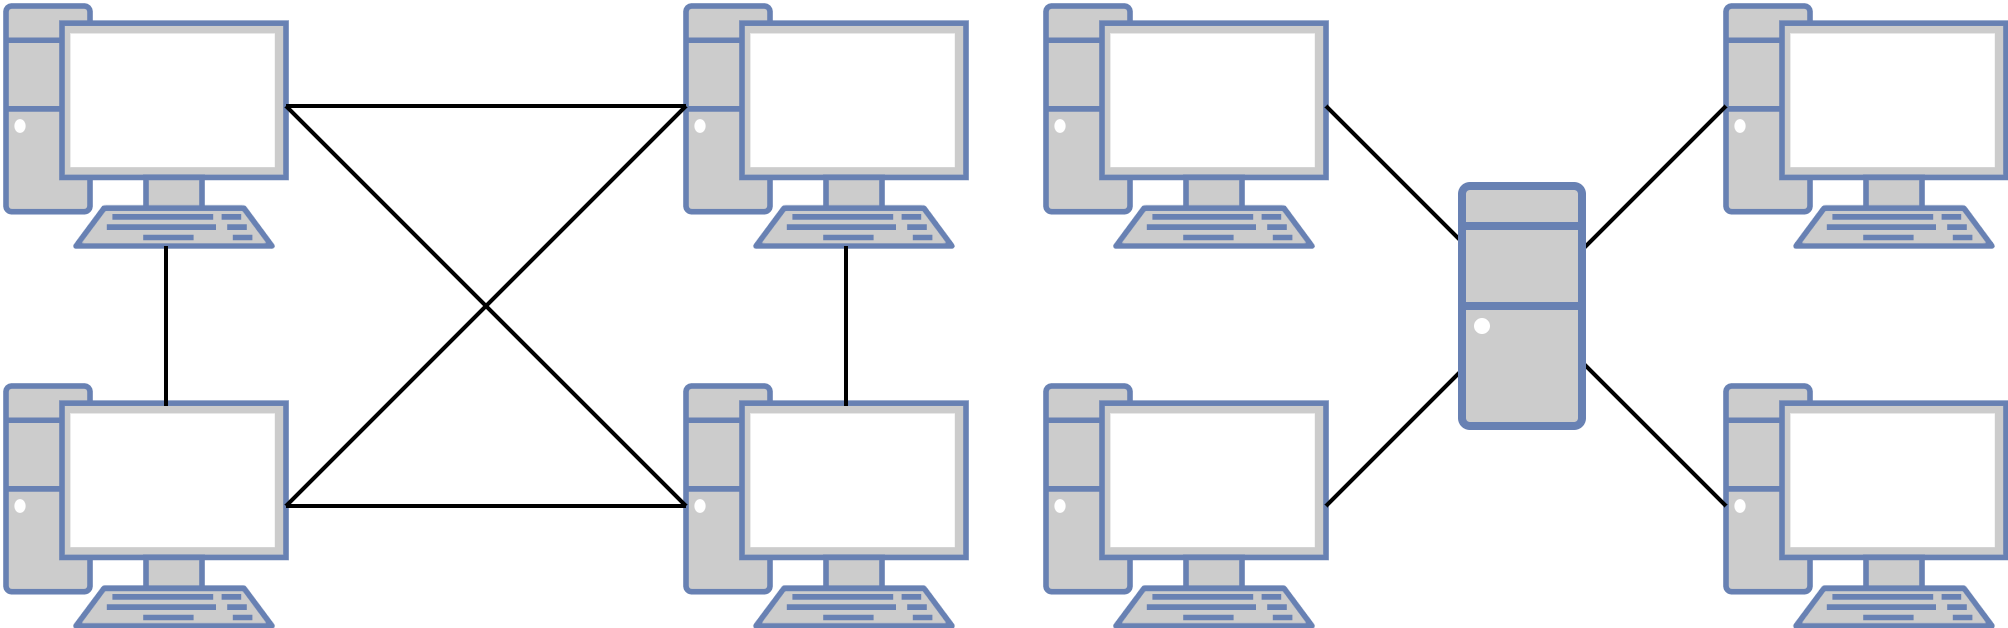
\includegraphics[scale=0.7]{images/Figure2.png}
	\end{center}
	\vspace{-0.6cm}
	\caption{P2P network and client-server network.}
	\label{fig:fig2}
\end{figure}

\noindent
Peers are creating a sense of virtual community. This community of peers can resolve greater tasks, beyond those that individual peers can do. Yet, these tasks are beneficial to all the peers in the system~\cite{BandaraJ13}. When a request comes to such a network, a node that accepted request is usually called \textbf{coordinator}, because he then is trying to found the right peer to send a request to.

Based on how the nodes are linked to each other within the overlay network, and how resources are indexed and located, we can classify networks as~\cite{KamelSE07}:

\begin{itemize}
	\item \textbf{Unstructured} do not have a particular structure by design, but they are formed by nodes that randomly form connections~\cite{FilaliBHB11}. Their strength and weakness at the same time is the lack of structure. These networks and robust when peers join and leave the network. But when doing a query, they must found more possible peers that have the same piece of data. A typical example of this group is a Gossip-based protocol like~\cite{DasGM02}.
	\item \textbf{Structured} peers are organized into a specific topology, and the protocol ensures that any node can efficiently search the network for a resource. The famous type of structured P2P network is a Distributed Hash Table (DHT). These networks maintain lists of neighbors to do a more efficient lookup, and as such, they are not so robust when nodes join or leave the network. DHT commonly used in resource lookup systems~\cite{StoicaMKKB01}, and as efficient resource lookup management and scheduling of applications, or as an integral part of distributed storage systems and NoSQL\cite{Leavitt10} databases.
	\item \textbf{Hybrid} combine the previous two models in various ways.
\end{itemize}

\noindent
P2P networks are a great tool in many arsenals, but because of their unique ability to act as a server and as a client at the same time, we must be aware and pay more attention to security because they are more vulnerable to exploits~\cite{0024003}.
%
%
\subsection{Master-slave}\label{sec:master_slave}
%
In the master-slave architecture, there is one node that is in charge -- \textbf{master}. This node accepts requests, and we usually do not communicate to the rest of the nodes or \textbf{slaves}. The master node is usually better and more expensive or even specialized hardware such as RAID drives to lower the crash probability. The cluster can also be configured with a \textbf{standby} master, and this node is continually updated from the master node.

But no matter how specialized hardware master runs on, it is prone to fail for various reasons, so he is a \textbf{single point of failure}. If crush happened, then standby master could continue to the server as a master, or new \textbf{leader election} protocol~\cite{KorachKM90} is initiated to pick a new master node. 

The master node is responsible for processing any updates to that data. If the master fails, then the slaves can still handle \textbf{read} requests. Failure of the standby master node, to take over from the master node is a real problem if we want to achieve a high-availability system.

Figure~\ref{fig:fig16} show difference between mater-slave $(left)$ and peer-to-peer $(right)$ request handling.

\begin{figure}[H]
	\begin{center}
		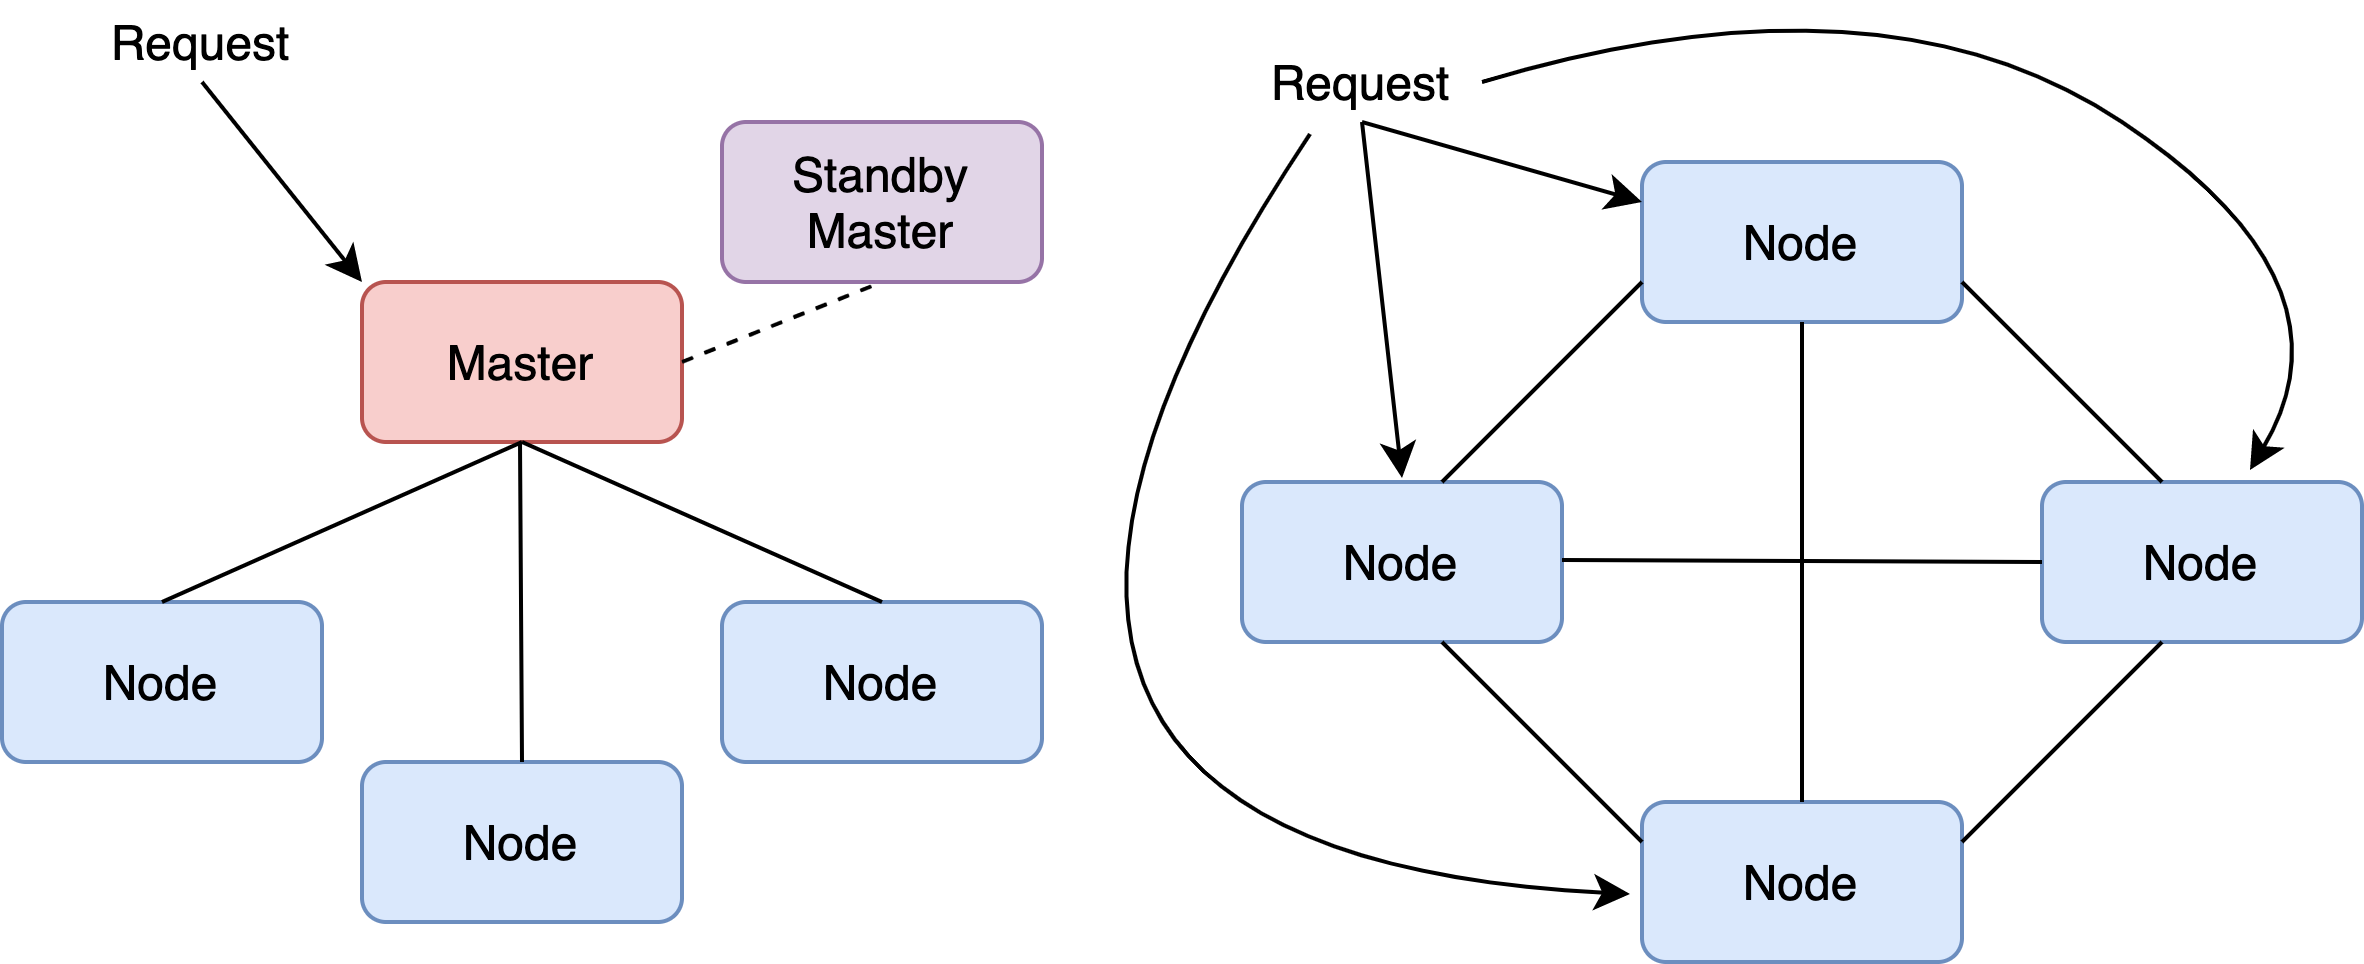
\includegraphics[scale=0.7]{images/Figure16.png}
	\end{center}
	\vspace{-0.6cm}
	\caption{Handling requests master-slave and peer-to-peer}
	\label{fig:fig16}
\end{figure}

\noindent
Using the right distribution model usually depends on the business requirements. High availability requires a P2P network because no single point of failure. If we could manage data using batch jobs that run in off-hours, then the simpler master-slave model might be the solution.
%
%
\section{Similar computing models}\label{sec:similar_models}
%
In this section, we are going to shortly describe models that are similar to the DS, and as such, they may be the source of confusion.
%
%
\subsection{Parallel computing}\label{sec:parallel_computing}
%
DC and parallel computing seem like models that are the same, and that may share some features like simultaneously executing a set of computations in parallel. Broadly speaking, this is not far from the truth~\cite{Vera16}. 

Distinguished between the two can be presented as follows: in parallel computing, all processor units have access to the shared memory and have some way of the faster inter-process communication, while in DS and DC all processors have their memory on their machine and communicate over the network to other nodes which are significantly slower. 

These models are similar, but they are not identical, and the kinds of problems they are designed to work on are different. Figure~\ref{fig:fig4} visually summarize the architectural  differences between DC $(up)$ and parallel computing $(down)$.

\begin{figure}[H]
	\begin{center}
		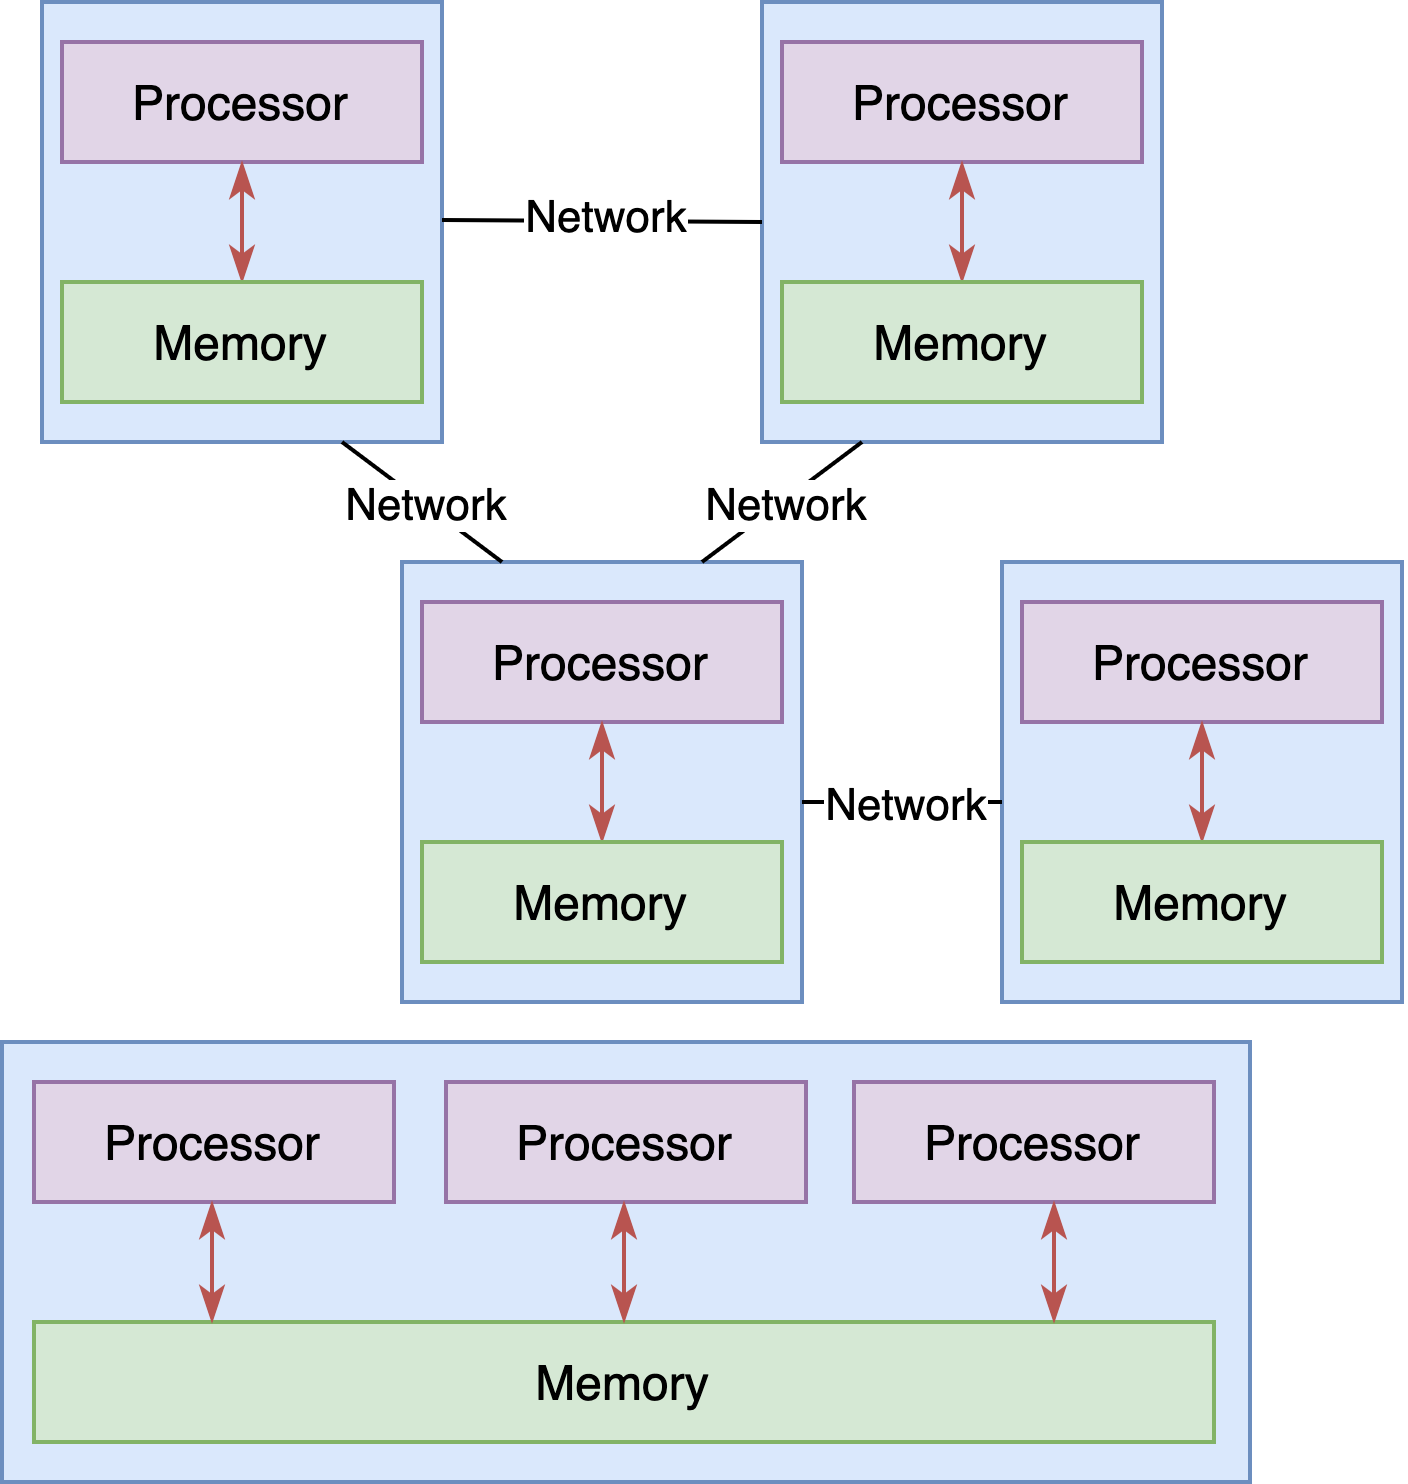
\includegraphics[scale=0.8]{images/Figure4.png}
	\end{center}
	\vspace{-0.6cm}
	\caption{Architectural difference between DC and parallel computing.}
	\label{fig:fig4}
\end{figure}

\noindent
Parallel computing has often used the strategy with problems, that due to their nature or constraints must be done on multi-core machines simultaneously~\cite{0072397}. It is often, that some big problems are divided into smaller ones, which can then be solved at the same time. 

Several tasks require parallel computing like simulations, computer graphics rendering, or different scenarios in scientific computing.
%
%
\subsection{Decentralized systems}\label{sec:decentralized_systems}
%
Decentralized systems are similar to DS, in a technical sense, they are still DS. But if we take a closer look, these systems \textbf{should not} be owned by a single entity. CC, for example, is a perfect example of DS, but it is not decentralized by its nature. It is a centralized system by the owner like AWS, Google, Microsoft, or some other private company because all computation needs to be moved to big DCs~\cite{HossainRH18}.

By modern standards, when we are talking about decentralized systems, we usually think of blockchain or blockchain-like technology~\cite{LeibleSSG19}. Since here we have distributed nodes, that are scattered and there is no single entity that owns all these nodes. But even if this technology is run in the cloud, it is losing the decentralized feature. This is the caveat we need to be aware of. These systems are facing different issues because any participant in the system might be malicious and they need to handle this case. 

Nonetheless, CC can and should be decentralized in the sense that some computation can happen outside of cloud big DCs, closer to the sources of data. These computations could be owned by someone else, and big cloud companies could give their solution to this as well to relax centralization and problems that CC will have especially with ever-growing IoT and mobile devices.
%
%
\section{Virtualization techniques}\label{sec:virtualization_techniques}
%
Virtualization as a technique started long ago in time-sharing systems, to provide isolation between multiple users sharing a single system like a mainframe computer~\cite{CrosbyB06}. 

In~\cite{Sharma} Sharma et al. describe virtualization as technologies that provide a layer of abstraction of the physical computing resources between computer hardware systems and the software systems running on them.

Modern virtualization differentiates few different tools. Some of them are used as an integral part of the infrastructure for some flavors like IaaS, while others are used in different CC flavors as well as microservices packaging and distribution format, or are new and still are looking for their place. These options are:

\begin{itemize}
	\item \textbf{Virtual machines (VM)} are the oldest technology of the three. In~\cite{Sharma} Sharma et al. describe them as a self-contained operating environment consisting of guest operating system and associated applications, but independent of the host operating system. VMs enable us to pack isolation and better utilization of hardware in big DCs. They are widely used in IaaS environment~\cite{AbsalomBJ13, YangHCLW13} as a base where users can install their own operating system (OS) and required software tools and applications.
	\item \textbf{Containers} provide the almost same functionality to VMs, but there are several subtle differences that make them a goto tool in modern development. Instead of the guest OS running on top of host OS, containers use tools that are in a Linux kernel like \textit{cgroups} that limits process resource usage so that single process can not starve other processes and use all the resources for himself, and \textit{namespaces} to provide isolation and partitions kernel resources so that single process see node resources like he only exists there. Containers reduce time and footprint from development to testing to production, and they utilize even more hardware resources compared to VMs and show better performance compared to the VMs~\cite{Seo2014PerformanceCA, FelterFRR15}. Containers provide an easier way to pack services and deploy and they are especially used in microservices architecture and service orchestration tools like Kubernetes~\cite{BurnsGOBW16}. Google stated few times in their on-line talks that they have used container technology for all their services, even they run VMs inside containers for their cloud platform. Even though they exist for a while, containers get popularized when companies like Docker and CoreOS developed user-friendly APIs.
	\item \textbf{Unikernels} is the newest addition to the virtualization space. In~\cite{pavlicek2016unikernels} Pavlicek define unikernels as small, fast, secure virtual machines that lack operating systems. Unikernels are comprised of source code, along with only the required system calls and drivers. Because of their specific design, they have a single process and they contain and execute what it absolutely needs to nothing more and nothing less~\cite{GoethalsSAVT18}. They are advertised that new technology that will save resources and that they are \textit{green}~\cite{208735} meaning they save both power and money. When put to the test and compared to containers they give interesting results~\cite{GoethalsSAVT18, PlauthFP17}. Unikernels are still a new technology and they are not widely adopted yet. But they give promising features for the future, especially \textbf{if} properly ported to ARM architectures, and various development languages. Unikernels will probably be used as a user applications and functions virtualization tool, because of their specific architecture, especially for serverless applications presented in~\ref{sec:microservices}.
\end{itemize}

\noindent
With every virtualization technique, the ultimate goal is to pack as many applications on existing hardware as possible, so that there are no resources that are left not used -- we are trying to achieve high resource utilization. Figure~\ref{fig:fig5} represent architectural differences between VMs, containers, and unikernels.

\begin{figure}[H]
	\begin{center}
		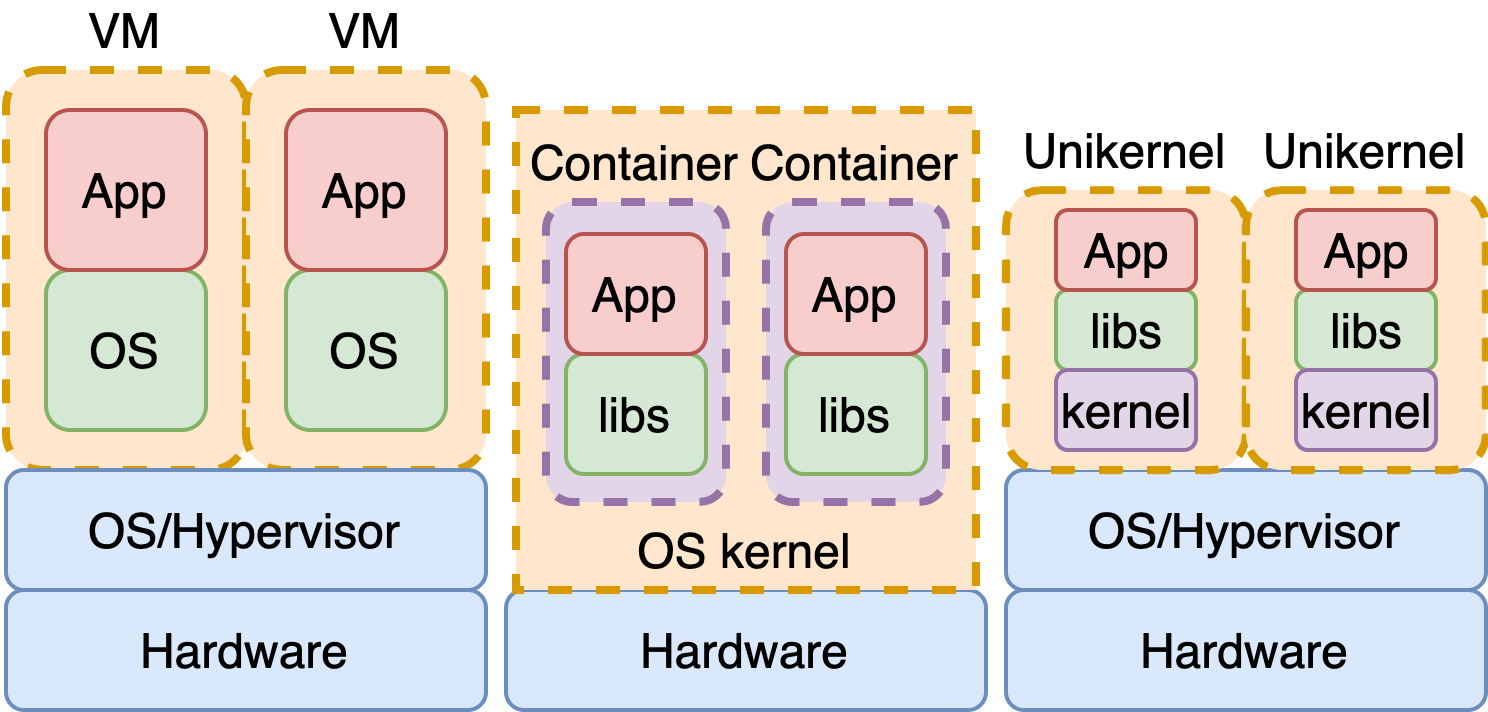
\includegraphics[scale=0.9]{images/Figure5.png}
	\end{center}
	\vspace{-0.6cm}
	\caption{Architectural differences between VMs, containers and unikernels.}
	\label{fig:fig5}
\end{figure}
%
%
\section{Deployment}\label{sec:deployment}
%
Over the years two different approaches evolved how to deploy infrastructure and applications. The difference just gets more amplified, when CC and microservices get into the picture, where frequent deployment is very common. 

Here evolve a new strategy to manage and deploy complicated infrastructure elements -- Infrastructure as code (IaC). In his book~\cite{wittig2018amazon} Wittig et al. describe it as a process of managing and provisioning computer data centers through machine-readable definition files, rather than physical hardware configuration or interactive configuration tools.

Deployments in such complex environment can be separated how they handle changes on existing infrastructure or applications on:

\begin{itemize}
	\item \textbf{Mutable model}, is a model where we have in place changes which mean that the parts of the existing infrastructure or applications get updated or changed to do an update. In place, change can produce few problems: $(1)$ more risk because in-place change may not finish which puts our infrastructure or the application in a possible bad state. This is especially a problem if we have a lot of services and multiple copies of the same service. The possibility that our system is not on is a lot higher, $(2)$ high complexity, this is a direct implication of the previous feature. Since our change might not get fully done, we cannot give a guarantee that our infrastructure or application is transitioned from one version to another -- change is not \textbf{descrete}, but \textbf{continues} since we might end up in some state in between where we are now and where we want to be.
	\item \textbf{Immutable model}, is a model where we do not do any in-place changes on existing infrastructure or application whatsoever. In this model, we replace it completely with a new version that is updated or changed compared to the previous version. The previous version gets discarded in favor of the new version. Compared to the previous model, immutable deployment has: $(1)$ less risk, since we do not change existing infrastructure or the application but we start a new one with and shut down the previous one. This is important especially in DS where everything can fail at any time, $(2)$ previous property reduces the complexity of the mutable deployment model. This is a direct implication of the previous feature, since we shut down and fully replace the previous version with the new one we get \textbf{descrete} version change and atomic deployment with deferring deployments with fast rollback and recovery processes. On the other hand, this process requires more resources~\ref{Helland16}, since both versions must be present on the node for this process is done. The second problem is data that is used by the application, we should not lose the data that the application is generated. If we externalize data then this problem is resolved. We should not rely on local storage but store that data elsewhere, especially when the parts of the system are volatile and changed often. The key advantage of this approach is avoiding downtime experienced by the end-user when new features are released.
\end{itemize}

\noindent
Figure~\ref{fig:fig12} summarize difference bewteen prevous infrastructure deplyment models.

\begin{figure}[H]
	\begin{center}
		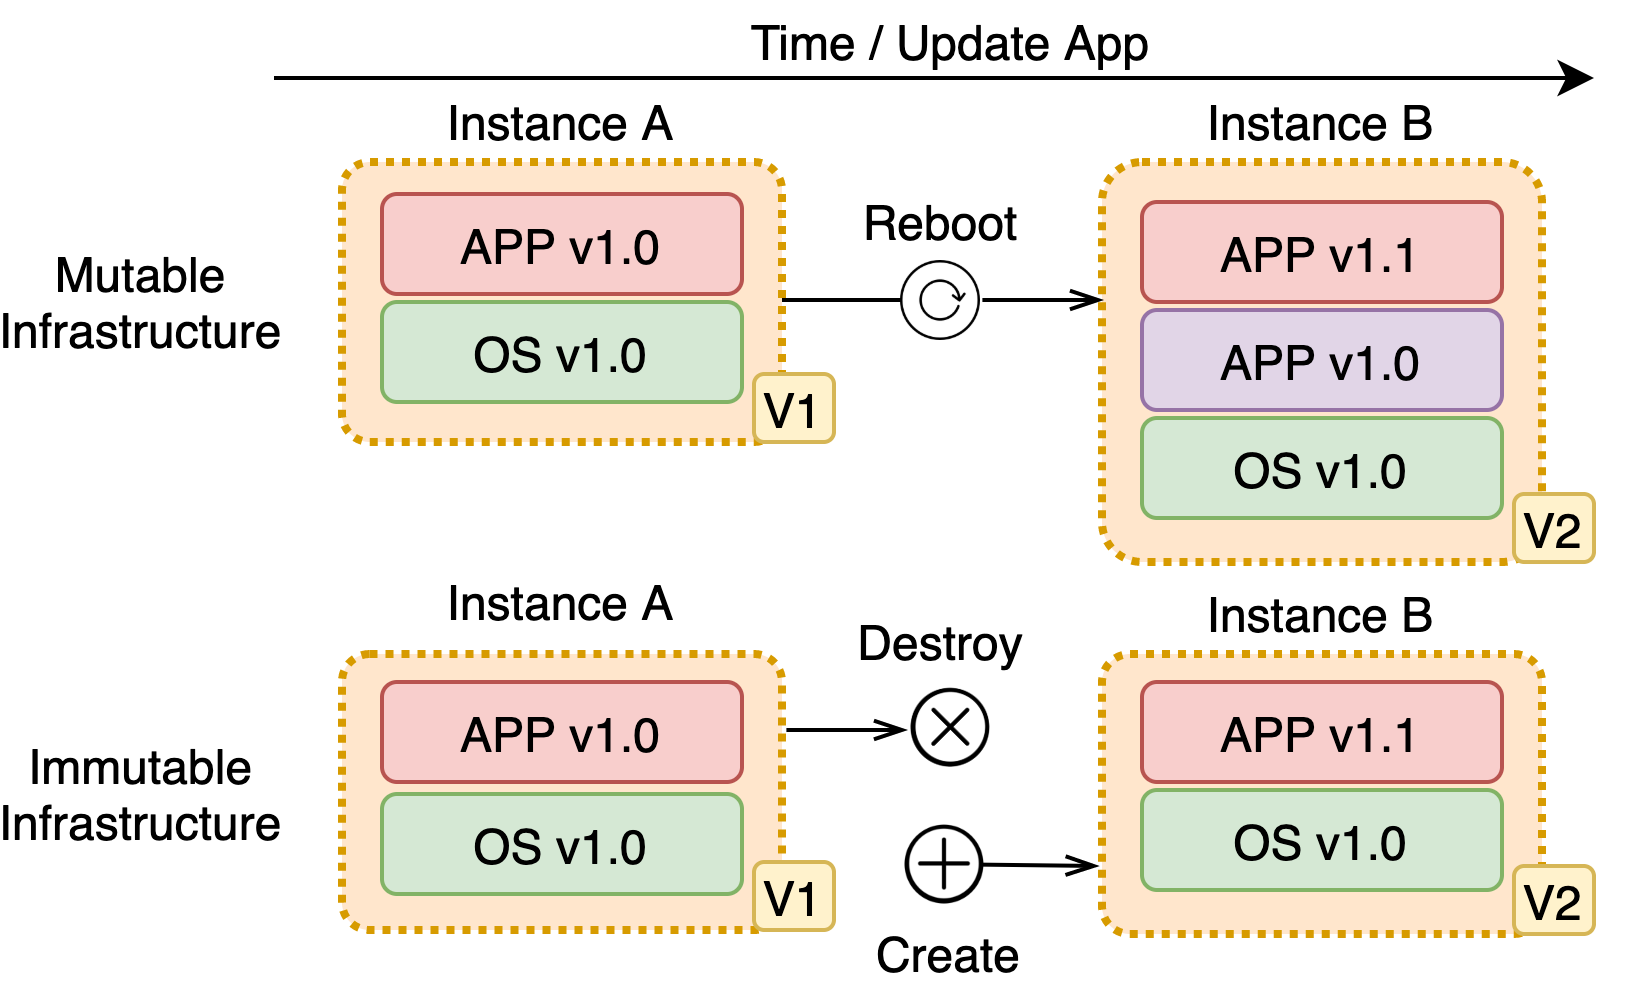
\includegraphics[scale=0.9]{images/Figure12.png}
	\end{center}
	\vspace{-0.6cm}
	\caption{Difference bewteen mutable and immutable deplyment models}
	\label{fig:fig12}
\end{figure}

Immutability is a simple concept to understand and simplify a lot especially in DS~\cite{Helland16}. Write down some data, and ensure that it never changes. It can never be modified, updated, or deleted~\cite{perry2020art}. When this is combined with the promise that we can avoid downtime especially in complex DS, it is clear why the immutable model is gaining more and more popularity (especially with the arrival of containers). Immutable infrastructure deployment offers few models on how to deploy change on the services, even in production to test it or switch to the whole new version. These strategies include:

\begin{itemize}
	\item \textbf{Blue-Green deployment}, this strategy require two separate environments: $(1)$ \textit{Blue} current running version, and $(2)$ \textit{Green} is the new version that needs to be deployed. When we are satisfied that the green version is working properly, we can gradually reroute the traffic from the old environment to the new environment for example by modifying DNS. This strategy offers near-zero downtime.
	\item \textbf{Canary update} is the strategy where we do direct a small number of requests to the new version --- the canary. If we are satisfied with the change, we can continue to increase the number of requests and monitor how the service is working with increasing load, monitor for errors, etc.
	\item \textbf{Rolling update} strategy update large environments a few nodes at a time. The setup is similar to blue-green deployment, but here we have a single environment. With this strategy, the new version gradually replaces the old one. But this is not the only benefit. If for whatever reason, the new version is not working properly on the larger amount of nodes, we can always do rolling back to the previous version.
\end{itemize}

\noindent
With mutable infrastructure, these strategies would be hard to implement, and maybe it is not possible at all. Besides infrastructure deployment, there is another side that we must consider, and that is how to describe these deployments. Here we can consider two different strategies:

\begin{itemize}
	\item \textbf{Imperative}, with this option users, have to write code or specific instructions step by step on what specific tool need to do so that the application or infrastructure is properly setup. In this approach, we have a \textit{smart} user who describes \textit{dumb} machine what is needed to be done and in what order to achieve the desired state.
	\item \textbf{Declarative}, with this option user, has to describe the end state or what is his desired state, and the tool needs to figure out the way how to do this. Here we have \textit{smart} system that will found a way how to achieve the desired state, and we have user who\textit{do not care} in what order actions need to be done --- that is what the system needs to do. Users do not need to worry about timing, this simplifies the whole process and the code always represents the latest state. With this type of deployment, we can offer users two different models: $(1)$ use existing formats that are user familiar with like JSON, YAML, XML, etc., or $(2)$ create a new domain-specific language that users need to learn, but we might be able to optimize description.
\end{itemize}

\noindent
With the introduction of \textit{LinuxKit}, we can create Linux subsystems based around very secure containers. With linuxkit, every part of the Linux subsystem is running inside the container, so we can assemble a Linux subsystem with services that are needed. As a result, systems created with LinuxKit have a smaller attack surface~\cite{abs-1802-10375} than general-purpose systems. This is important from the security point of view, but also infrastructure deployment because we can compose specific OS based around containers that we need for a different purpose. And we can update, change and adopt these OS for every machine or purpose we need.

Deployment is based around changing parts of the OS, and his services that are running inside containers. As a result, everything can be removed or replaced. It's highly portable and can work on desktops, servers, IoT, mainframes, bare metal, and virtualized systems.
%
%
\section{Concurency and parallelism}\label{sec:concurency_parallelism}
%
People usually confuse these two concepts. Even they look similar, they are a different way of doing things. In his talk, Rob Pike~\cite{Pike} give great explanation and examples on this topic. In his talk, he gives great definitions of these concepts like:

\begin{itemize}
	\item \textbf{Concurrency} is composition of independently executing things. Concurrency is about dealing with a lot of things at once.
	\item \textbf{Parallelism} is the simultaneous execution of multiple things. Parallelism is about doing a lot of things at once. 
\end{itemize}

\noindent
These things are important, especially when building applications and systems that should achieve very high throughput. We must build them with a good structure and a good concurrency model. These features enable possible parallelism, but with communication~\cite{Pike}. These ideas are based on Tony Hoare work of Communicating Sequential Processes (CSP)~\cite{Hoare78}.

\subsection{Actor model}\label{sec:actor_model}
%
An actor model, the main idea is based around \textbf{actors} which are small concurrent code, that communicate independently by sending messages, removing the need for lock-based synchronization~\cite{Hewitt}. This model proposes a similar idea to Tony Hoare in his work with CSP~\cite{Hoare78}, and actors are often confused with CSP. Table~\ref{tab:table6} give differences between actor model and CSP.

\begin{table}[h!]
	\begin{center}
		\begin{tabular}{l|l|l}
			\textbf{Feature} & \textbf{CSP} & \textbf{Actor model}\\
			\hline
			\textbf{Fault tolerance} & Distributed Queue &  Supervisors hierarchy \\
			\textbf{Process identity} & Anonymus & Concrete \\
			\textbf{Composition} & NA & Applicable \\
			\textbf{Communication} & Queue & Direct \\
			\textbf{Message passing} & Sync & Async\\
		\end{tabular}
	\end{center}
	\vspace{-0.5cm}
	\caption{Ddifferences between actor model and CSP.}
	\label{tab:table6}
\end{table}

Actors do not share a memory, and they are isolated by nature. An actor can create another actor/s and even watch on them in case they stop unexpectedly. And when an actor finished his job, and he is not needed anymore, it disappears. These actors can create complicated networks that are easy to understand, model, and reason about, and everything is based on a simple message passing mechanism. 

Every actor has a designated message box. When a message arrives, the actor will test the message type and do the job according to the message type he received. In this way, we are not dependent on lock-based synchronization that can be hard to understand, and it can cause serious problems.

The actor model is fault-tolerant by design. It supports crush to happen because there is a \say{self-heal} mechanism that will monitor actor/s, and when the crash happens it will try to apply some strategy, in most cases just restart actor, but other strategies could be applied. This philosophy is useful because it is hard to think about every single failure option.
%
%
\section{Motivation and Problem Statement}\label{sec:problem_statement}
%
In their work~\cite{GreenbergHMP09} Greenberg et al. point out that micro data-centers (MDCs) are used primarily as nodes in content distribution networks and other \say{embarrassingly distributed} applications.

One size rarely suits all needs, so the CC should not be our final computing shift. Various models presented in~\ref{sec:mobile_computing} show a promising possibility of how computing could be done closer to the data sources, to lower the latency for its clients by contacting the cloud only when needed. While the heavy computation could remain in the cloud, because of more available resources. Send to the cloud only information that is crucial for other services or applications~\cite{inproceedingsSimic1}. Not ingest everything as the standard cloud model proposes.

A zonally-based organization of servers combined with MDCs shows a great possibility for building micro-clouds and EC as a service. To achieve such a behavior, we need a few more abstractions and layers, to make the whole system more available, resilient, and with less latency. By their nature, EC originates from P2P systems~\cite{LopezMEDHIBFR15} as suggested by L{\'{o}}pez et al., but expands it into new directions and blends it with the CC. This very interesting, because we already have much research and knowledge available for P2P systems that we could use for inspiration. But one extension of the P2P system leads to geo-distributed deployments, and going from node to node is a time-consuming process. Satyanarayanan et al. stated that infrastructure deployment will not happen until the whole process is relatively easy~\cite{SatyanarayananBCD09}. 

If we assume that we have a well-defined system and the previous task is solved so that we can easily deploy infrastructure and operate with it, we will have a system that could be offered like any other resource in the CC -- as a service. Such a system or service could be offered to various types of users, from researchers to developers to create new types of applications. A well-defined system that is easy to operate with, will be able to move resources from one place to another with no problem. We also must be aware, that some cloud providers might choose to integrate the system into their existing CC platform to reduce the load or avoid bottlenecks and single points of failure~\cite{JararwehDAAAB16}.

The idea of small-scale servers introduced by EC, with heterogeneous, compute, storage, and network resources, raise interesting research ideas and it is the main motivation for this thesis. Taking advantage of resources organized locally as micro clouds, community clouds, or edge clouds~\cite{RydenOCW14} suggested by Ryden et al., to help power-hungry servers reduce traffic~\cite{HirschMZ18}. Contact the cloud only when needed~\cite{inproceedingsSimic1}. Send to the cloud only information that is crucial for other services or applications. Not ingest everything as the standard CC model proposes.

To achieve such behavior, dynamic resource management, and device management is essential. At any given time, we must know available resources, configuration, and utilization~\cite{GubbiBMP13, WangZZWYW17} of the system. Traditional DCs is a well organized and connected system, built upon years of experience. On the other hand, these MDCs consist of various devices, including ones presented in~\ref{sec:mobile_computing} that are not~\cite{JiangCGZW19}. This idea brings us to the problem this thesis address.

Currently, existing EC and MDCs models lack dynamic well defined geo-organization structure, native applications model, and a clear separation of concerns model. As such they cannot be offered as a service to the users, and it is hard to form micro-clouds on them. Usually, these systems exist independently from one another, scattered without any communication between them. Providers who build and maintain these systems, usually lock users in their ecosystem frequently integrate tightly with their cloud services giving users small or even no other options. Nearby EC nodes could be organized locally, making the whole system more available and reliable, but at the same time extending resources beyond the single node or group of nodes, maintaining good performance to build servers and clusters~\cite{ArocaG12}.

This cloud extension strengthens our understanding of not just DS but also CC as a system and field of research. With EC native applications model, separation of concerns well defined, and a unified node organization strategy, we are moving towards the idea of EC as a service and micro-clouds. Based on this, we define the problem this thesis is trying to solve, through the three research questions:

\begin{enumerate}[start=1,label={(\bfseries \arabic*)}]\label{questions}
	\item \textit{Can we organize geo-distributed EC nodes in a similar way to the cloud, but adopted for the different environment, with clear separation of concerns and familiar applications model for users forming micro-cloud a model?}
	\item \textit{Can we offer these organized nodes (micro-clouds) as a service based on the cloud pay as you go model, to the developers and researchers so that they can develop new human-centered applications?}
	\item \textit{Can we make a model in such a way that is formally correct, easy to extend, understand and reason about?}
\end{enumerate}

\noindent
This micro-cloud model makes both system and applications more available and reliable, while resources are extended further beyond the single node or even MDCs. IN his work~\cite{SatyanarayananK19} Satyanarayanan et al. show that MDCs can serve as firewalls, while users get a unique ability to dynamically and selectively control their information that will be uploaded to the cloud.  Simi\' c et al., in~\cite{inproceedingsSimic1} use a similar idea as a pre-processing tier for the cloud. Years after its inception, EC is no longer just an idea~\cite{SatyanarayananK19} but a must-have tool for novel applications to come. 
%
%
\section{Research Hypotheses, and Goals}\label{sec:research_hyphotesis_and_golas}
%
Based on research questions presented on a page~\pageref{questions}, and motivation presented in a section~\ref{sec:problem_statement}, we derive the hypotheses around which we base this thesis. We can summarize them as follows:

\begin{enumerate}[start=1,label={(\bfseries \arabic*)}]
	\item \textbf{Hypothesis:} \textit{It is possible to organize EC nodes in a standard way based on cloud architecture, adapted for EC geo-distributed environment -- \textbf{micro-clouds}. Giving users the unique ability to organize nodes, descriptively, in the best possible way to serve the only population nearby.}
	\item \textbf{Hypothesis:} \textit{It is possible to offer a newly formed micro-cloud model to researchers and developers as a service based on the cloud pay as you go model to create new human-centered applications. But sustain the ability to rearrange resources as needed.}
	\item \textbf{Hypothesis:} \textit{It is possible to form a clear separation of concerns for the future micro-cloud model (EC as a service model) and establish a well-organized system with an intuitive role for every part.} 
	\item \textbf{Hypothesis:} \textit{It is possible to present a unified model that will be able to support heterogeneous small-scale servers (EC nodes). This unified model will rely on a set of technical requirements that nodes must fulfill to join the system.}
	\item \textbf{Hypothesis:} \textit{It is possible to present a clear and familiar application model so that users can use the full potential of newly created infrastructure but familiarly and intuitively.}
\end{enumerate}

\noindent
From the previously defined hypotheses, we can derive the primary goals of this thesis, where the expected results include:

\begin{enumerate}[start=1,label={(\bfseries \arabic*)}]
	\item \textit{The construction of a model with a clear separation of concerns for the model influenced by cloud organization, with adaptations for a different environment. With a model for EC applications utilizing these adaptations. This addresses the first research question and is the topic of Chapter~\ref{chapter:Micro_clouds}.}
	\item \textit{The constructed model is more available, resilient with less latency, and as such it can be offered to the general public as a service like any other service in the cloud. This addresses the second research question and is the topic of Chapter~\ref{chapter:Micro_clouds}.}
	\item \textit{The constructed model is described formally well, using solid mathematical theory, but also easy to extend both formally and technically, easy to understand and reason about. This addresses the third research question and is the topic of Chapter~\ref{chapter:Micro_clouds}.}
\end{enumerate}
%
%
\section{Structure of the thesis}\label{sec:structure_of_thesis}
%
Throughout this introductory Chapter, we defined the motivation for our work with problems that this thesis addresses and presented the necessary background information and areas to support our work. Here we outline the rest of the thesis.

Chapter~\ref{chapter:Review} presents the literature review, where we examine different aspects of existing systems and methods important for the thesis. We analyze existing organizational abilities for nodes in both industry and academia frameworks and solutions to address our first research question. We further examine platform models from industry and academia tools and frameworks to address our second research question. And last but not least, we examine current strategies to offload tasks from the cloud. All three parts address our third research question.

Chapter~\ref{chapter:Micro_clouds} details our model, how it is related to other research and where it connects to other existing models and solutions. We further describe our solution as well as protocols required for such a system to be implemented formally. We give examples of how existing infrastructure could be used, as well as familiar application model for developers. 

Chapter~\ref{chapter:Implementation} presents implementation details of a framework developed to test hypotheses defined earlier in this chapter, but also a model and formally defined protocols defined in~\ref{chapter:Micro_clouds}. This chapter also shows results after conducting experiments, current limitations of the implemented system, and possible applications that could benefit from such a system.

Chapter~\ref{chapter:Conclusion} concludes our work and presents opportunities for further research and development.
%
%